\documentclass[12pt]{article}
\usepackage{graphicx}
\usepackage{placeins}


% acronyms for text or math mode
\newcommand {\ccast} {\mbox{\small CCAST}}
\newcommand {\cris} {\mbox{\small CrIS}}

\newcommand {\airs} {\mbox{\small AIRS}}
\newcommand {\iasi} {\mbox{\small IASI}}
\newcommand {\idps} {\mbox{\small IDPS}}
\newcommand {\nasa} {\mbox{\small NASA}}
\newcommand {\noaa} {\mbox{\small NOAA}}
\newcommand {\nstar} {\mbox{\small STAR}}
\newcommand {\umbc} {\mbox{\small UMBC}}
\newcommand {\uw}   {\mbox{\small UW}}

\newcommand {\fft}  {\mbox{\small FFT}}
\newcommand {\ifft} {\mbox{\small IFFT}}
\newcommand {\fir}  {\mbox{\small FIR}}
\newcommand {\fov}  {\mbox{\small FOV}}
\newcommand {\for}  {\mbox{\small FOR}}
\newcommand {\ict}  {\mbox{\small ICT}}
\newcommand {\ils}  {\mbox{\small ILS}}
\newcommand {\igm}  {\mbox{\small IGM}}
\newcommand {\opd}  {\mbox{\small OPD}}
\newcommand {\rms}  {\mbox{\small RMS}}
\newcommand {\zpd}  {\mbox{\small ZPD}}
\newcommand {\ppm}  {\mbox{\small PPM}}
\newcommand {\srf}  {\mbox{\small SRF}}
\newcommand {\sdr}  {\mbox{\small SDR}}

\newcommand {\ES} {\mbox{\small ES}}
\newcommand {\SP} {\mbox{\small SP}}
\newcommand {\IT} {\mbox{\small IT}}
\newcommand {\SA} {\mbox{\small SA}}

\newcommand {\ET} {\mbox{\small ET}}
\newcommand {\FT} {\mbox{\small FT}}

% abbreviations, mainly for math mode
\newcommand {\real} {\mbox{real}}
\newcommand {\imag} {\mbox{imag}}
\newcommand {\atan} {\mbox{atan}}
\newcommand {\obs}  {\mbox{obs}}
\newcommand {\calc} {\mbox{calc}}
\newcommand {\sinc} {\mbox{sinc}}
\newcommand {\psinc} {\mbox{psinc}}
\newcommand {\std} {\mbox{std}}

% symbols, for math mode only
\newcommand {\wn} {\mbox{cm$^{-1}$}}
\newcommand {\lmax} {L_{\mbox{\tiny max}}}
\newcommand {\vmax} {V_{\mbox{\tiny max}}}

\newcommand {\tauobs} {\tau_{\mbox{\tiny obs}}}
\newcommand {\taucal} {\tau_{\mbox{\tiny calc}}}
\newcommand {\Vdc}  {V_{\mbox{\tiny DC}}}

\newcommand {\rIT} {r_{\mbox{\tiny\textsc{ict}}}}
\newcommand {\rES} {r_{\mbox{\tiny\textsc{es}}}}
\newcommand {\robs} {r_{\mbox{\tiny obs}}}

\newcommand {\rITobs} {r_{\mbox{\tiny\textsc{ict}}}^{\mbox{\tiny obs}}}
\newcommand {\rITcal} {r_{\mbox{\tiny\textsc{ict}}}^{\mbox{\tiny cal}}}

\newcommand {\ITmean} {\langle\mbox{\small IT}\rangle}
\newcommand {\SPmean} {\langle\mbox{\small SP}\rangle}


\title{SECOND DRAFT \\
  \vspace{5mm}
  Deconvolution and Translation \\
  Between High Spectral Resolution  \\
  IR Sounders \\
}

\author{Howard E.~Motteler \\
  \\
  UMBC Atmospheric Spectroscopy Lab \\
  Joint Center for Earth Systems Technology \\
}

\date{\today}
\begin{document}

\maketitle

\section{Introduction}

Upwelling infrared radiation as measured by the {\airs}, {\iasi},
and {\cris} sounders is a significant part of the long term climate
record.  We would like to treat this information as a single data
set but the instruments have different spectral resolutions, channel
response functions, and band spans.  As a first step in addressing
this problem we consider several channel radiance translations:
{\iasi} to high resolution {\cris}, {\iasi} to {\airs}, {\airs} to
standard resolution {\cris}, and high resolution {\cris} to {\airs}.

Translation from {\airs} to {\cris} presents a special challenge
because {\cris} and {\iasi} are Michaelson interferometers with
parametrized response functions, while {\airs} is a grating
spectrometer with channel center frequencies and spectral response
functions determined by the focal plane geometery.  In section
\ref{decon} we show how to take advantage of detailed knowledge of
the {\airs} spectral response functions (SRFs) to deconvolve {\airs}
channel radiances to a resolution enhanced intermediate
representation.

The translations presented here are validated by comparisons with
calculated reference truth.  For example to test the {\iasi} to
{\airs} translation, we start with 49 fitting profiles spanning a
significant range of atmospheric conditions.  Upwelling radiance is
calculated at a 0.0025 {\wn} grid with kcarta over a band spanning
the {\airs} and {\iasi} response functions.  ``True {\airs}'' is
calculated from this by convolving the kcarta radiances with {\airs}
SRFs, and ``true {\iasi}'' by convolving kcarta radiances to the
{\iasi} instrument specifications.  {\iasi} is translated to {\airs}
(we call this ``{\iasi} {\airs}'') and this is compared with true
{\airs}.

This sort of validation assumes perfect knowledge of the {\airs} and
{\iasi} instrument response functions and so gives only a lower bound
on residuals, and so on how well the translations can work in practice.
But the better we know the response functions, the closer practical
translations can approach these limits.  The conversions here are
presented in order of the residuals, with {\iasi} to high resolution
{\cris} most accurate and high resolution {\cris} to {\airs} the
least.  After the translation sections, the {\airs} deconvolution is
examined in greater detail.

This report is the theoretical basis document for the sounder
radiance translations implemented in the airs\_decon and iasi\_deon
git repositories, and is included in the airs\_decon repo.  It is
under development in parallel with the work there.  In addition to
the translations, the repositories include the test and validation
code used to produce the results shown here.  The repositories are
available at github,
\begin{verbatim}
  https://github.com/strow/airs_deconv.git
  https://github.com/strow/iasi_decon.git
\end{verbatim}


\section{IASI to high resolution CrIS}

The {\cris} user grid comprises three bands, LW 650 to 1095 {\wn},
MW 1210 to 1750 {\wn}, and SW 2155 to 2550 {\wn}.  For the {\cris}
high resolution mode the channel spacing is 0.625 {\wn} for all
three bands.  The {\cris} user ILS is a sinc function.  The {\iasi}
user grid is a single band from 645 to 2760 {\wn} with a channel
spacing of 0.5 {\wn}.  The {\iasi} user ILS is a sinc function
convolved with the modified Gaussian, shown in figure \ref{igauss}.

{\iasi} to {\cris} is an easy translation because {\iasi} spans the
{\cris} bands and has a nominal (though strongly apodized) higher
resolution.  The main steps, for each {\cris} band, are

\begin{itemize}

  \item apply a bandpass filter to the {\iasi} channel radiances to
    restrict them to a single {\cris} band with a rolloff outside the
    {\cris} user grid

  \item take the filtered radiances to an interferogram with an
    inverse Fourier transform

  \item apply the pointwise inverse of the {\iasi} Gaussian over the 
    {\iasi} 1~cm {\opd} and truncate this to the 0.8~cm {\cris} {\opd}.

  \item take the interferogram back to radiance at the {\cris}
    0.625 {\wn} channel spacing with a forward Fourier transform

\end{itemize}

For the first step the passband is the {\cris} user grid and the
rolloff the minimum of data available and 15 {\wn} for the LW, 20
{\wn} for the MW, and 22 {\wn} for the SW.  So for example for the 
LW band we use a 5 {\wn} rolloff because {\iasi} starts at 645 {\wn}.
The rolloff reduces ringing at the band edges.

Figure \ref{iclw1} shows the mean and standard deviation of {\iasi}
{\cris} minus true {\cris} for the 49 fitting profiles, for the
{\cris} LW band.  The residual is greatest at the low end of the LW
band.  The residual is reduced significantly if we apply Hamming
apodization to the {\iasi} {\cris} and true {\cris} radiances, as
shown in figure \ref{iclw2}.  Figures \ref{icmw1} and \ref{icsw1}
show similar results for the unapodized radiances for the MW and SW
bands. The residuals are very small.  Unless otherwise noted, all
{\cris} spectra shown here are unapodized.

% \newpage

\begin{figure}
  \centering
  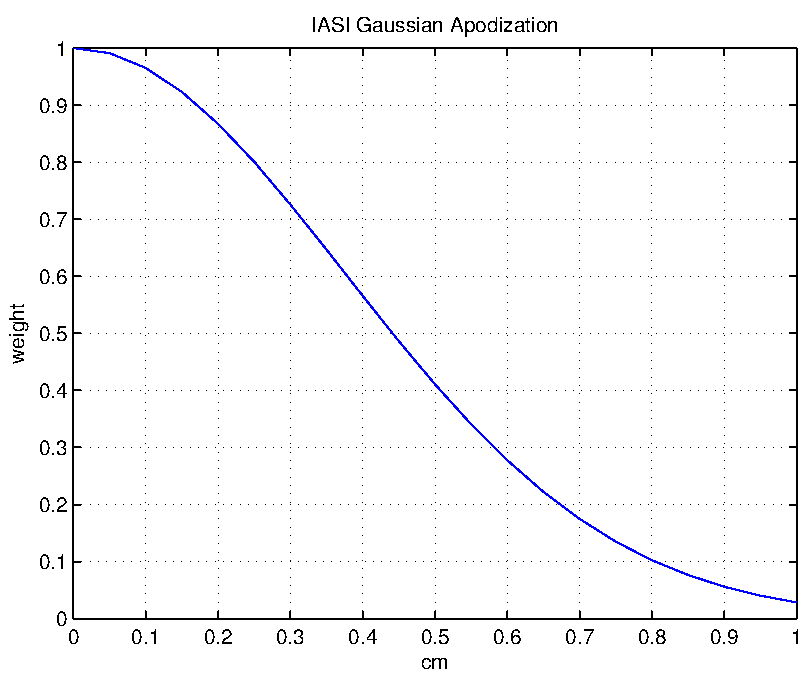
\includegraphics[height=8cm]{figures/iasi_gauss_app.pdf}
  \caption{{\iasi} truncated Gaussian apodization}
  \label{igauss}
\end{figure}

\begin{figure}
  \centering
  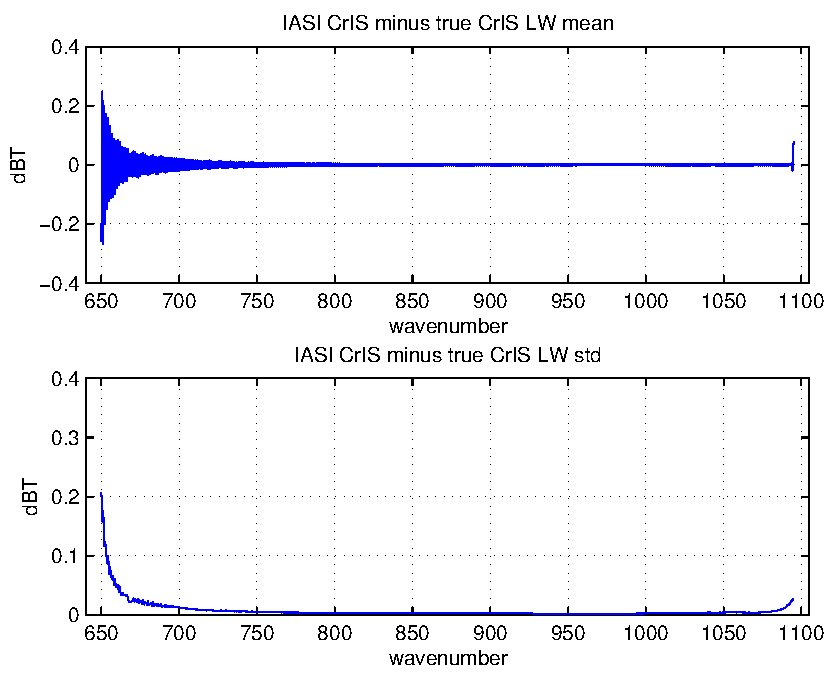
\includegraphics[height=8cm]{figures/iasi_cris_lw_1.pdf}
  \caption{Mean and standard deviation of unapodized {\iasi} {\cris}
    minus true {\cris}, for the {\cris} LW band.}
  \label{iclw1}
\end{figure}

\begin{figure}
  \centering
  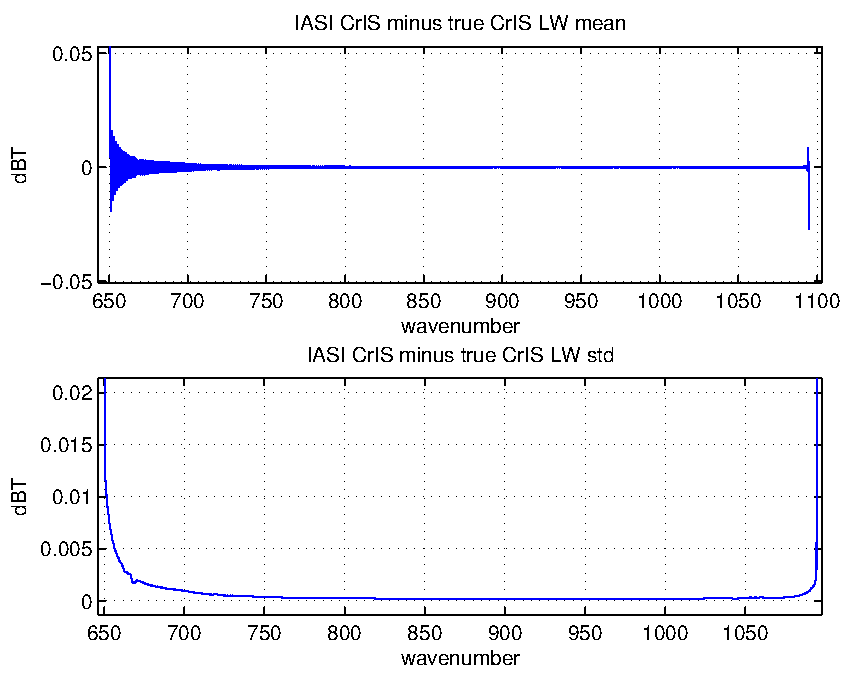
\includegraphics[height=8cm]{figures/iasi_cris_lw_2.pdf}
  \caption{Mean and standard deviation of Hamming apodized {\iasi}
    {\cris} minus true {\cris}, for the {\cris} LW band.}
% The residual is reduced by an order of magnitude
  \label{iclw2}
\end{figure}

\begin{figure}
  \centering
  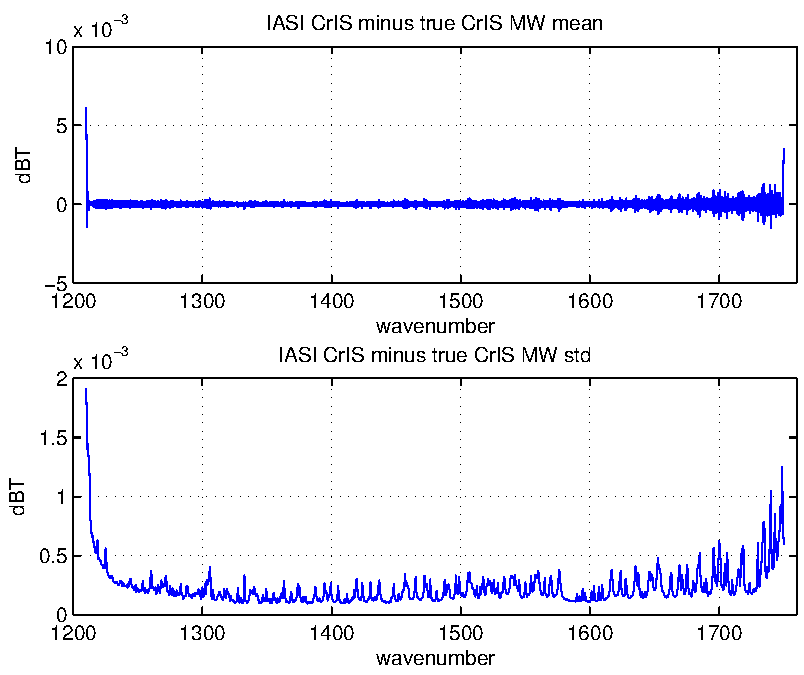
\includegraphics[height=8cm]{figures/iasi_cris_mw_1.pdf}
  \caption{Mean and standard deviation of unapodized {\iasi} {\cris}
    minus true {\cris}, for the {\cris} MW band.}
  \label{icmw1}
\end{figure}

\begin{figure}
  \centering
  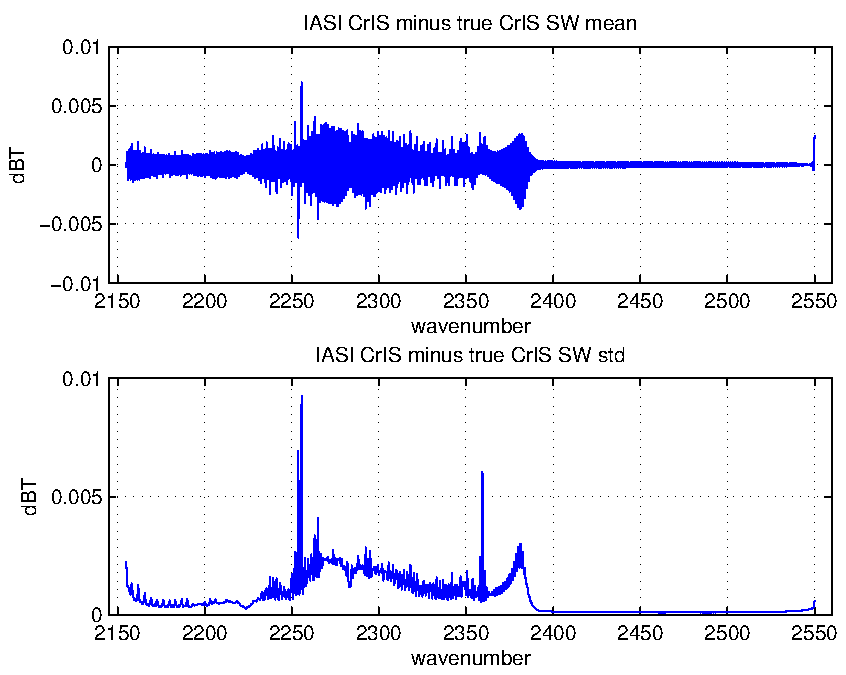
\includegraphics[height=8cm]{figures/iasi_cris_sw_1.pdf}
  \caption{Mean and standard deviation of unapodized {\iasi} {\cris}
    minus true {\cris}, for the {\cris} SW band.}
  \label{icsw1}
\end{figure}

\FloatBarrier


\section{IASI to AIRS}

{\airs} L1b radiances are a set of channels between approximately
650 to 2650 {\wn} with the individual center frequencies and
spectral response functions (SRFs) determined by the focal plane
geometery.  Channels are not uniformly spaced.  {\airs} L1c
radiances are derived from the L1b with improvements including a
more uniform spacing.  The {\iasi} to {\airs} translation works for
either channel set and is done as follows

% The {\iasi} to {\airs} translation applies a deconvolution to the
% full {\iasi} band, to a 0.1 {\wn} intermediate grid, and then an
% {\airs} convolution to get {\airs} channel radiances.  

\begin{itemize}

  \item apply a bandpass filter to the {\iasi} radiances to restrict
    them to the {\airs} band span, with a 5 {\wn} rolloff

  \item deconvolve the filtered {\iasi} radiances to a 0.1 {\wn}
    intermediate grid, the nominal resolution of the {\airs} SRF
    tabulation.  Aside from resolution and band spans, this exactly
    the same transform used for the {\iasi} to {\cris} translation
    and is done with the same procedure, iasi\_decon.m

  \item convolve the 0.1 {\wn} intermediate representation with either
    the {\airs} L1b or L1c SRFs.  Section \ref{decon} discusses this
    convolution in greater detail.
    
\end{itemize}

Figure \ref{srfs1} shows the first three {\airs} SRFs and the
bandpass filter wing.  Note the relatively gentle slope of the
rolloff, to decrease impulse ringing.  The first two {\airs} SRFs
are ``guard channels'' and the third the first regular channel.  
The wings of the SRFs roll off well inside the bandpass filter.

Figure \ref{iaspec} shows true {\iasi}, true {\airs}, deconvolved
{\iasi}, and {\iasi} {\airs}.  At this level of detail we mainly see
the greater fine structure in the deconvolution.  Figure \ref{iazoom}
shows details from 660 to 680 {\wn}.  Figure \ref{iadiff} shows
{\iasi} {\airs} minus true {\airs}.  The residual is larger than for
the {\iasi} to {\cris} translation, but significantly smaller than
for the {\airs} to {\cris} or {\cris} to {\airs} translations.

\begin{figure}
  \centering
  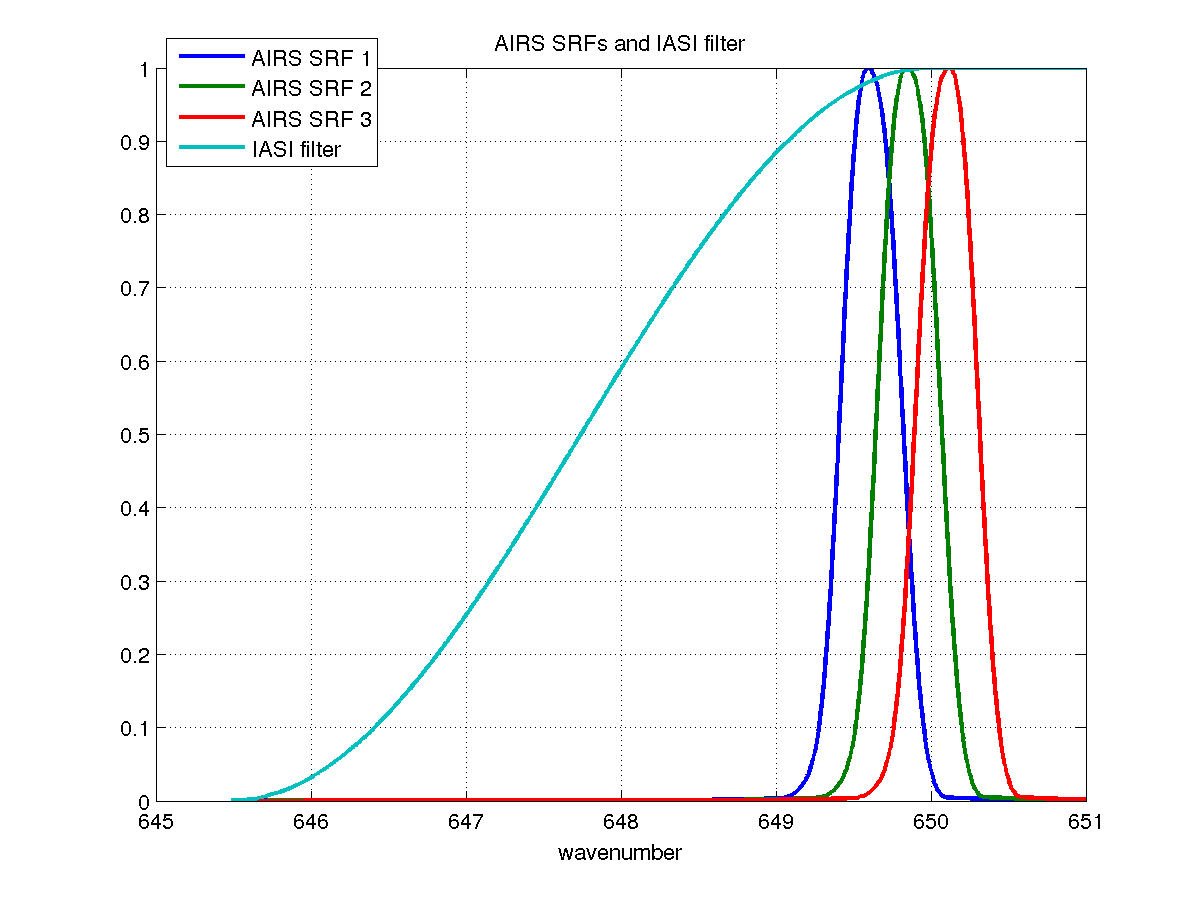
\includegraphics[height=8cm]{figures/srfs_and_filt.png}
  \caption{The first three {\airs} SRFs and the bandpass filter
    wing}
  \label{srfs1}
\end{figure}

\begin{figure}
  \centering
  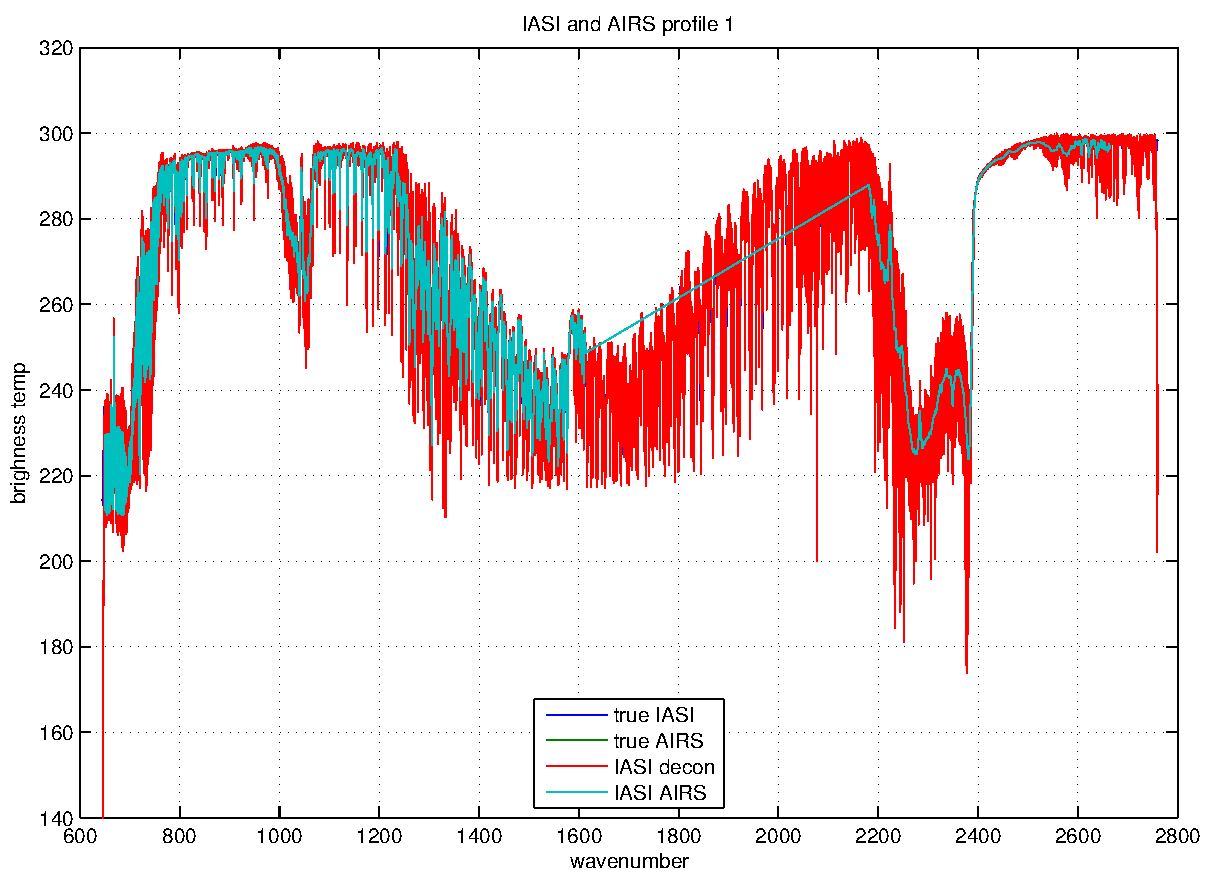
\includegraphics[height=8cm]{figures/iasi_airs_spec.pdf}
  \caption{true {\iasi}, true {\airs}, deconvolved {\iasi}, and
    {\iasi} {\airs} }
  \label{iaspec}
\end{figure}

\begin{figure}
  \centering
  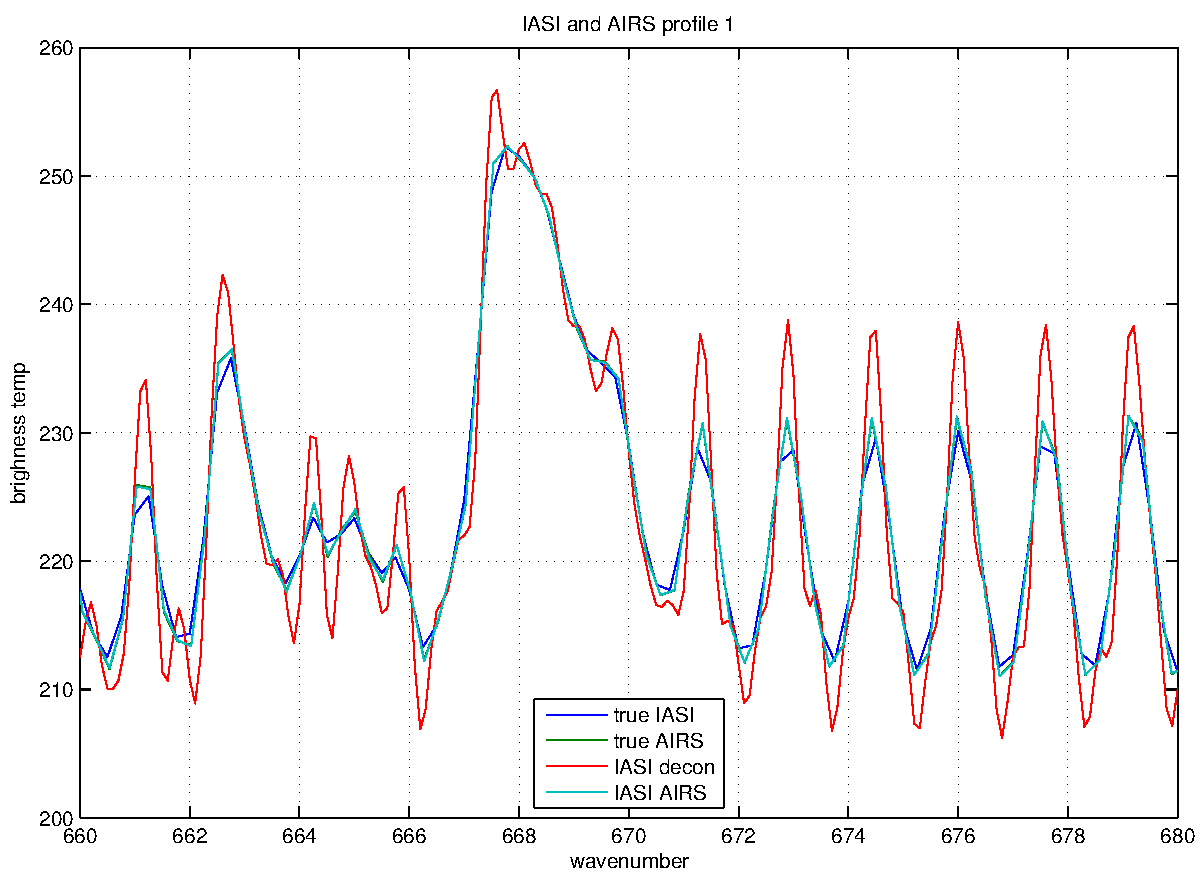
\includegraphics[height=8cm]{figures/iasi_airs_zoom.pdf}
  \caption{true {\iasi}, true {\airs}, deconvolved {\iasi}, and
    {\iasi} {\airs}, detail }
  \label{iazoom}
\end{figure}

\begin{figure}
  \centering
  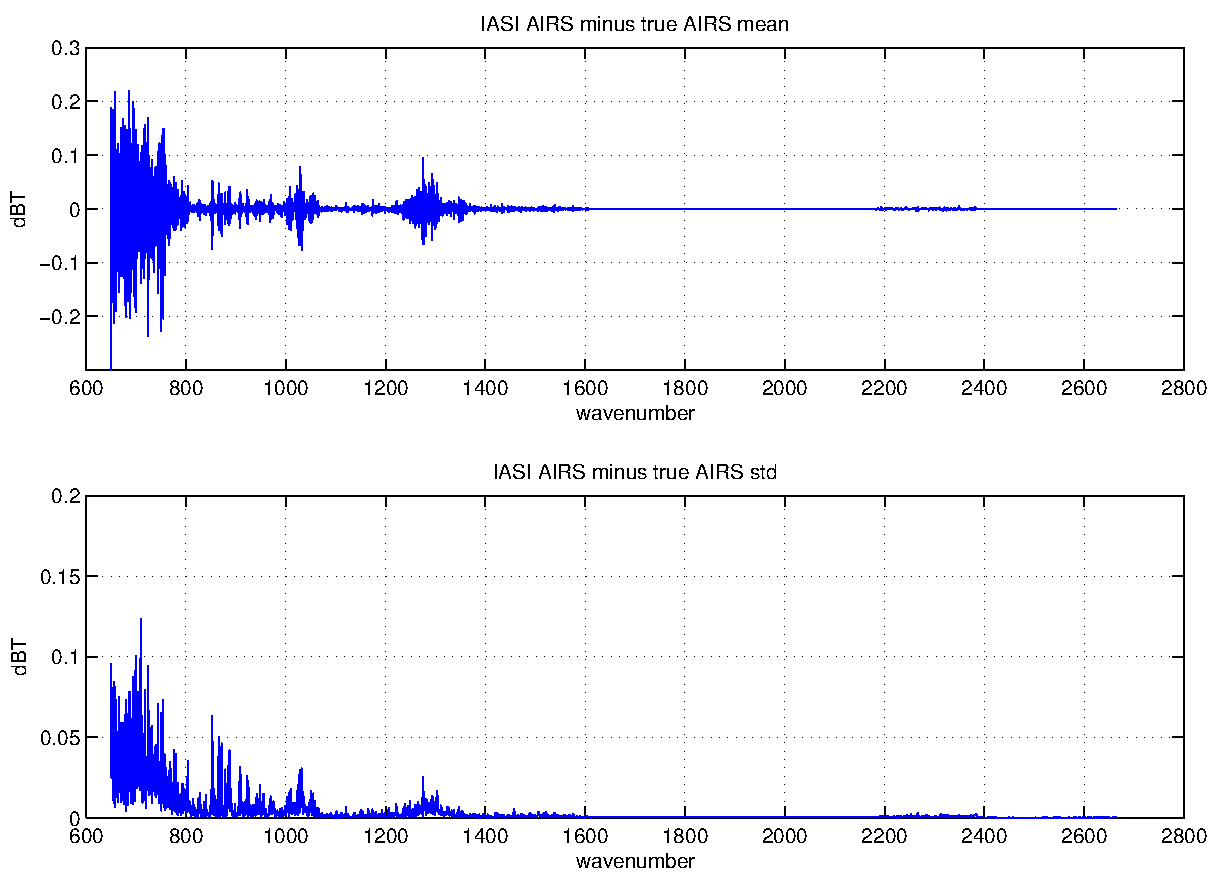
\includegraphics[height=8cm]{figures/iasi_airs_diff.pdf}
  \caption{Mean and standard deviation of {\iasi} {\airs} minus true
    {\airs} }
  \label{iadiff}
\end{figure}

\FloatBarrier

\section{AIRS to standard resolution CrIS}
\label{airs2cris}

For the {\cris} standard resolution mode the channel spacing is
0.625 {\wn} for the LW, 1.25 {\wn} for the MW, and 2.5 {\wn} for the
SW bands.  The {\iasi} deconvolution was the key step in the {\iasi}
to {\cris} and {\iasi} to {\airs} translations.  Similarly, {\airs}
deconvolution is central to the {\airs} to {\cris} translation and
is presented in detail in section \ref{decon}.  The first step in
the {\airs} L1c to {\cris} translation is to deconvolve the {\airs}
channel radiances to a 0.1 {\wn} intermediate grid, the nominal
{\airs} SRF resolution.  Then for each {\cris} band,

\begin{itemize}
  \item find the {\airs} and {\cris} band intersection

  \item apply a bandpass filter to the deconvolved {\airs} radiances
    to restrict them to the intersection, with a rolloff outside the
    intersection

  \item reconvolve the filtered spectra to the {\cris} user grid

\end{itemize}

Figure \ref{aclws} shows true {\cris}, true {\airs}, deconvolved
{\airs}, and {\airs} {\cris}.  At this level of detail we mainly see
the greater fine structure in the deconvolution.  Figure \ref{aclwz}
shows details from 660 to 680 {\wn}.  In comparison with the {\iasi}
deconvolution in figure \ref{iazoom} the {\airs} deconvolution is
not as smooth.  The remaining figures show true {\cris} minus
{\airs} {\cris} for the 49 fitting profiles, with and without
Hamming apodization for each of the {\cris} bands.  The residuals
are significantly reduced with apodization but are larger than for
the {\iasi} to {\cris} translation.

\begin{figure}
  \centering
  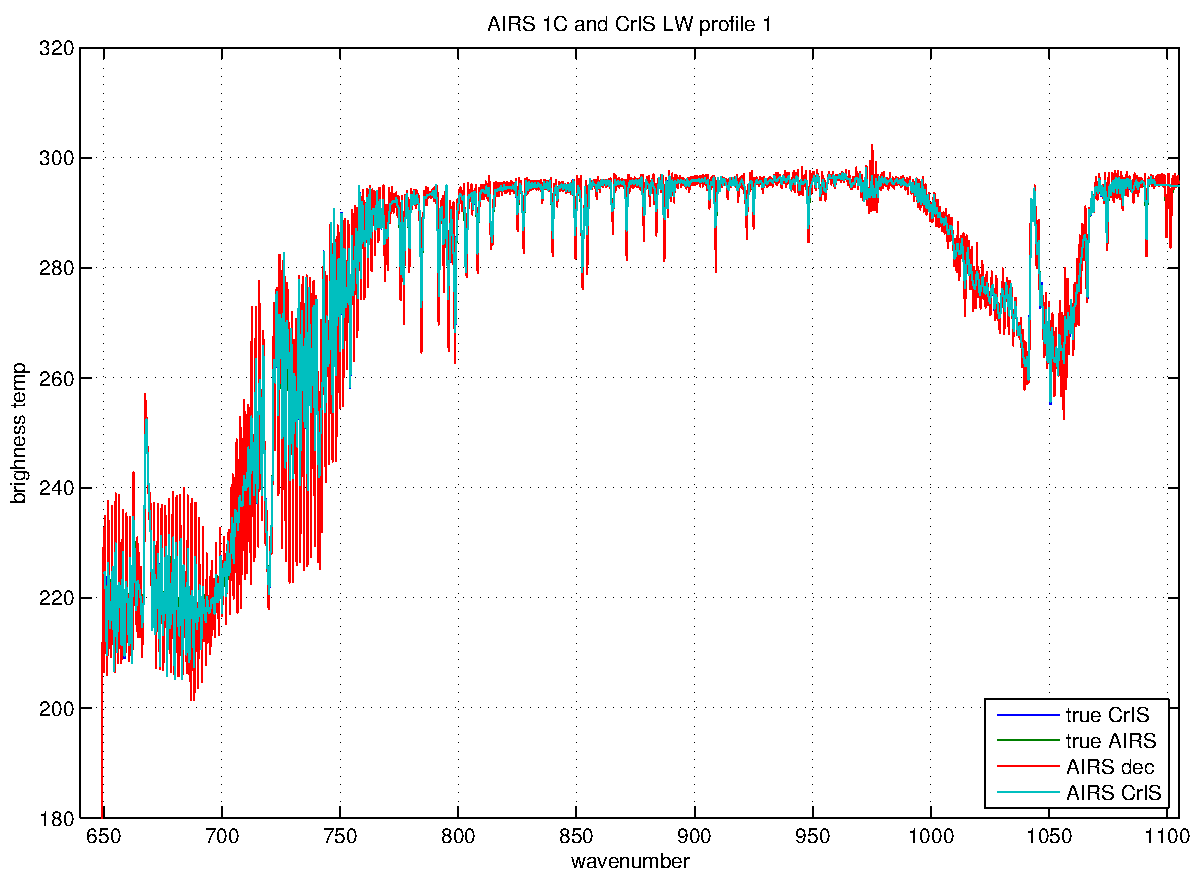
\includegraphics[height=8cm]{figures/airs_cris_spec_LW_noap.pdf}
  \caption{true {\cris}, true {\airs}, deconvolved {\airs}, and
    {\airs} {\cris} }
  \label{aclws}
\end{figure}

\begin{figure}
  \centering
  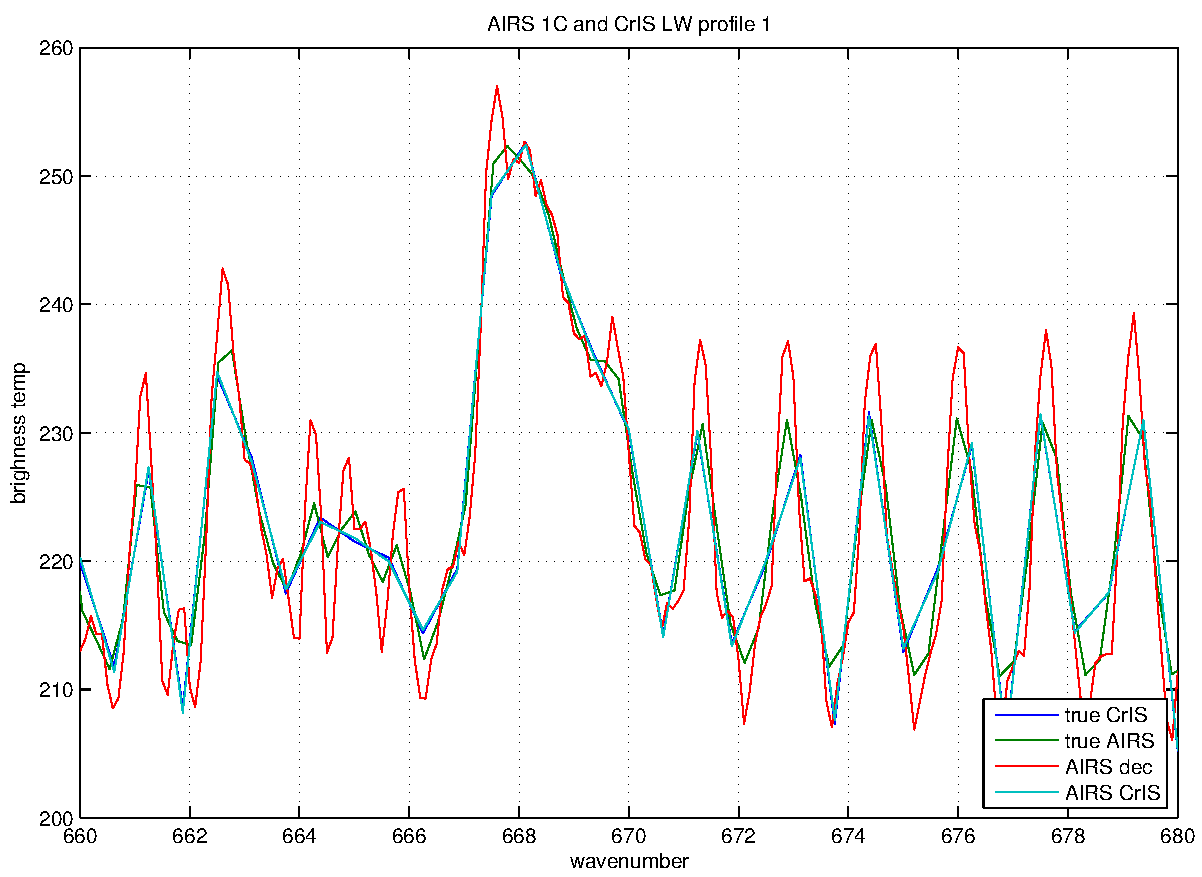
\includegraphics[height=8cm]{figures/airs_cris_zoom_LW_noap.pdf}
  \caption{true {\cris}, true {\airs}, deconvolved {\airs}, and
    {\airs} {\cris}, detail }
  \label{aclwz}
\end{figure}

% \begin{figure}
%   \centering
%   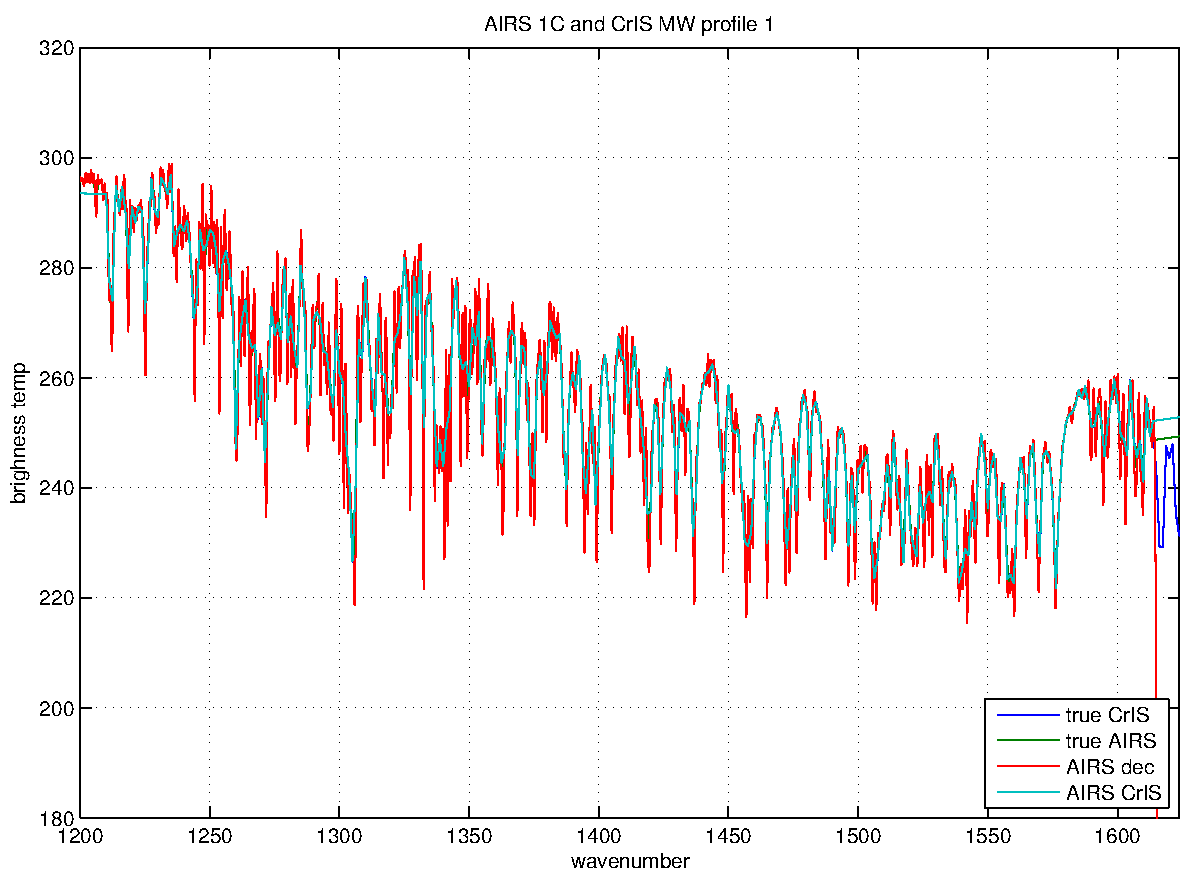
\includegraphics[height=8cm]{figures/airs_cris_spec_MW_noap.pdf}
%   \caption{ }
%   \label{acmws}
% \end{figure}

% \begin{figure}
%   \centering
%   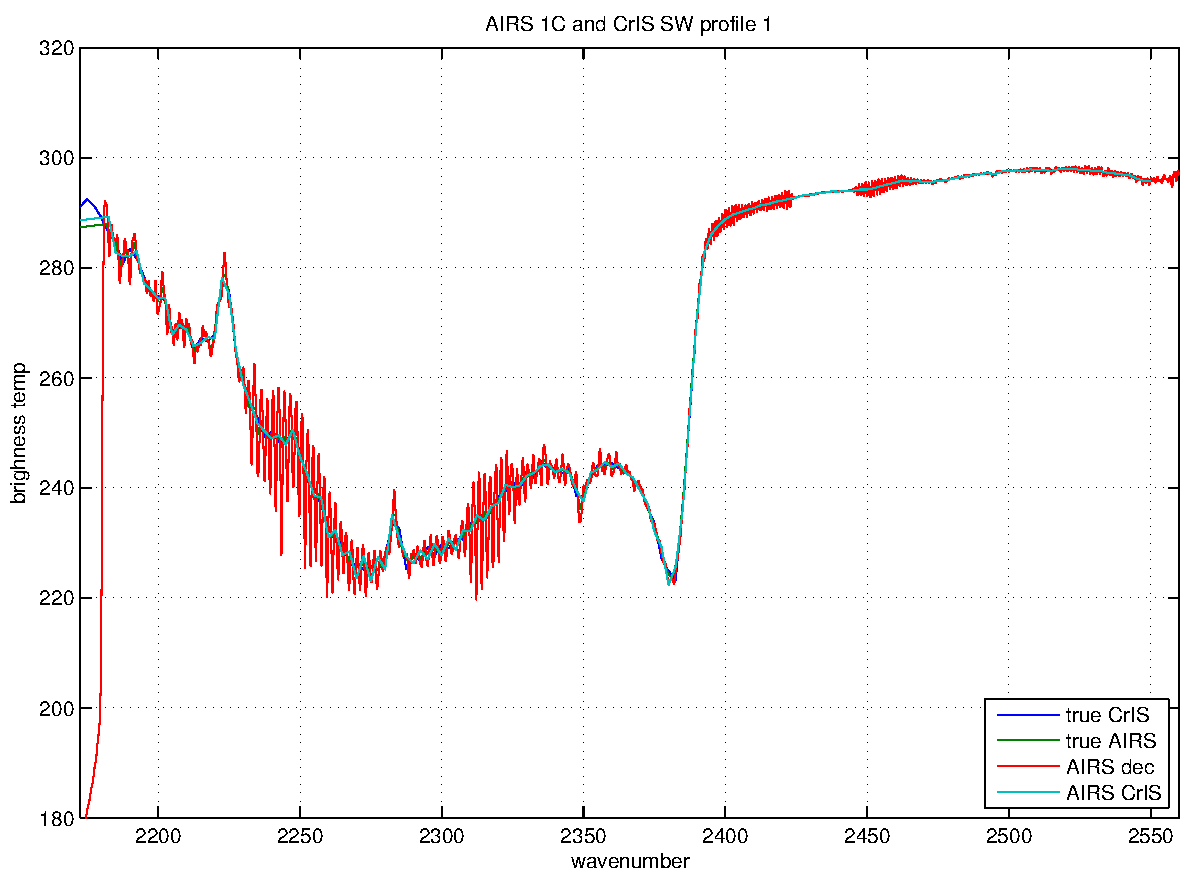
\includegraphics[height=8cm]{figures/airs_cris_spec_SW_noap.pdf}
%   \caption{ }
%   \label{acsws}
% \end{figure}

\begin{figure}
  \centering
  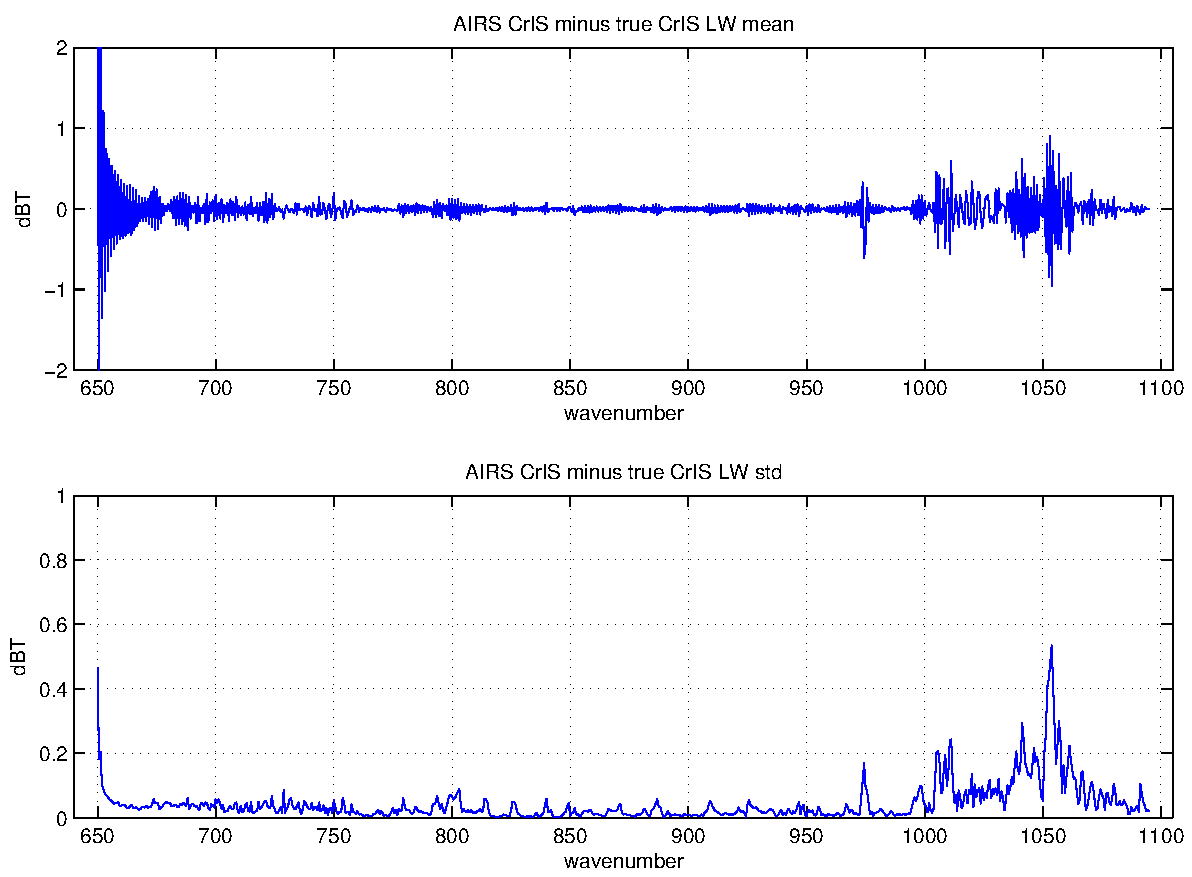
\includegraphics[height=8cm]{figures/airs_cris_diff_LW_noap.pdf}
  \caption{Mean and standard deviation of unapodized {\airs} {\cris}
    minus true {\cris}, for the {\cris} LW band }
  \label{aclwd}
\end{figure}

\begin{figure}
  \centering
  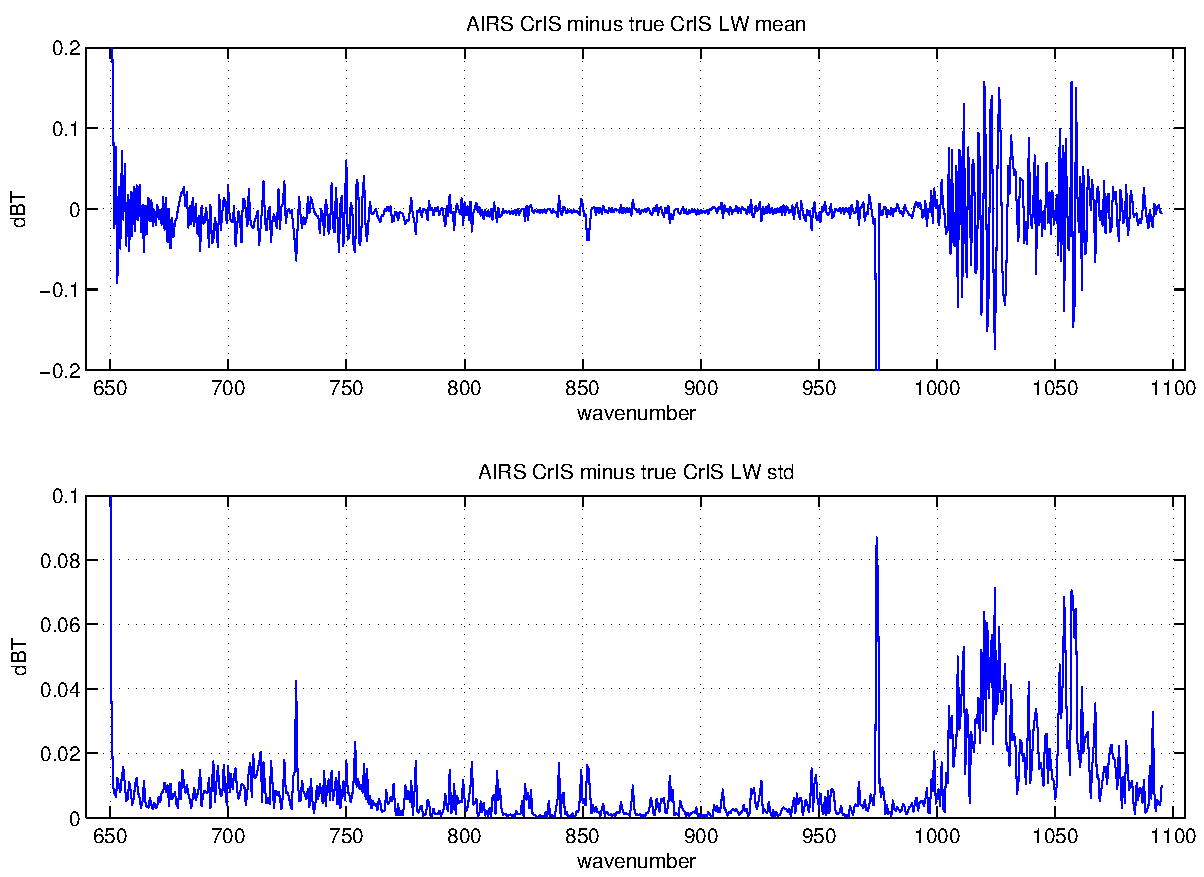
\includegraphics[height=8cm]{figures/airs_cris_diff_LW_hamm.pdf}
  \caption{Mean and standard deviation of Hamming apodized {\airs}
      {\cris} minus true {\cris}, for the {\cris} LW band }
  \label{aclwdh}
\end{figure}

\begin{figure}
  \centering
  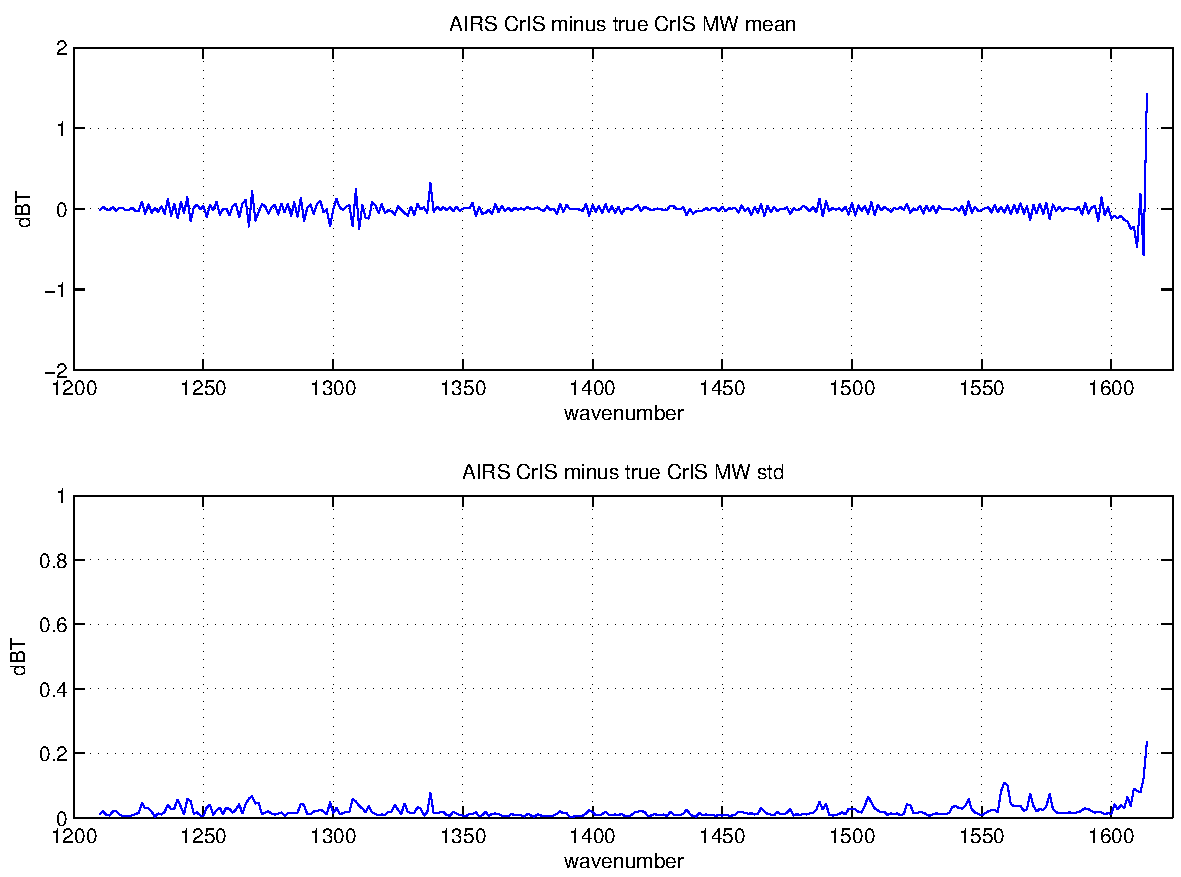
\includegraphics[height=8cm]{figures/airs_cris_diff_MW_noap.pdf}
  \caption{Mean and standard deviation of unapodized {\airs} {\cris}
    minus true {\cris}, for the {\cris} MW band }
  \label{acmwd}
\end{figure}

\begin{figure}
  \centering
  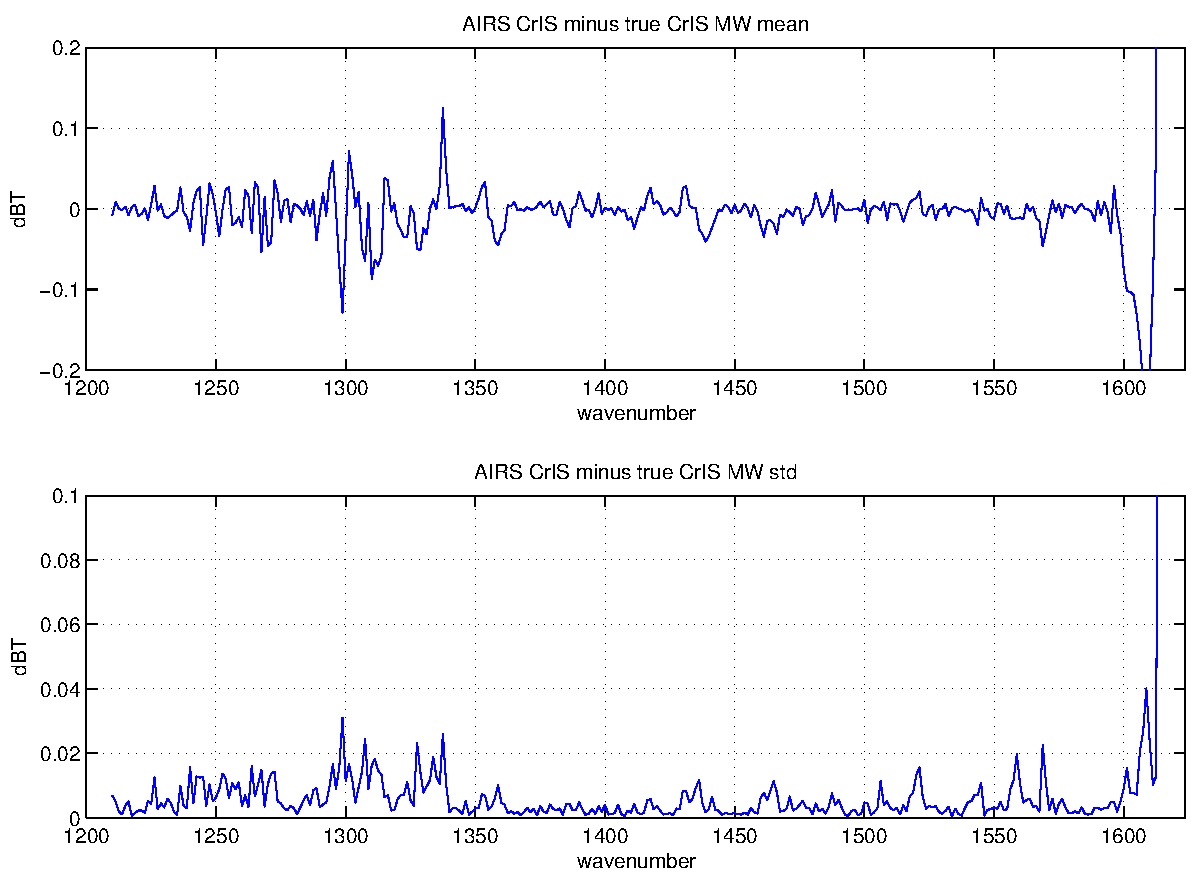
\includegraphics[height=8cm]{figures/airs_cris_diff_MW_hamm.pdf}
  \caption{Mean and standard deviation of Hamming apodized {\airs}
      {\cris} minus true {\cris}, for the {\cris} MW band }
  \label{acmwdh}
\end{figure}

\begin{figure}
  \centering
  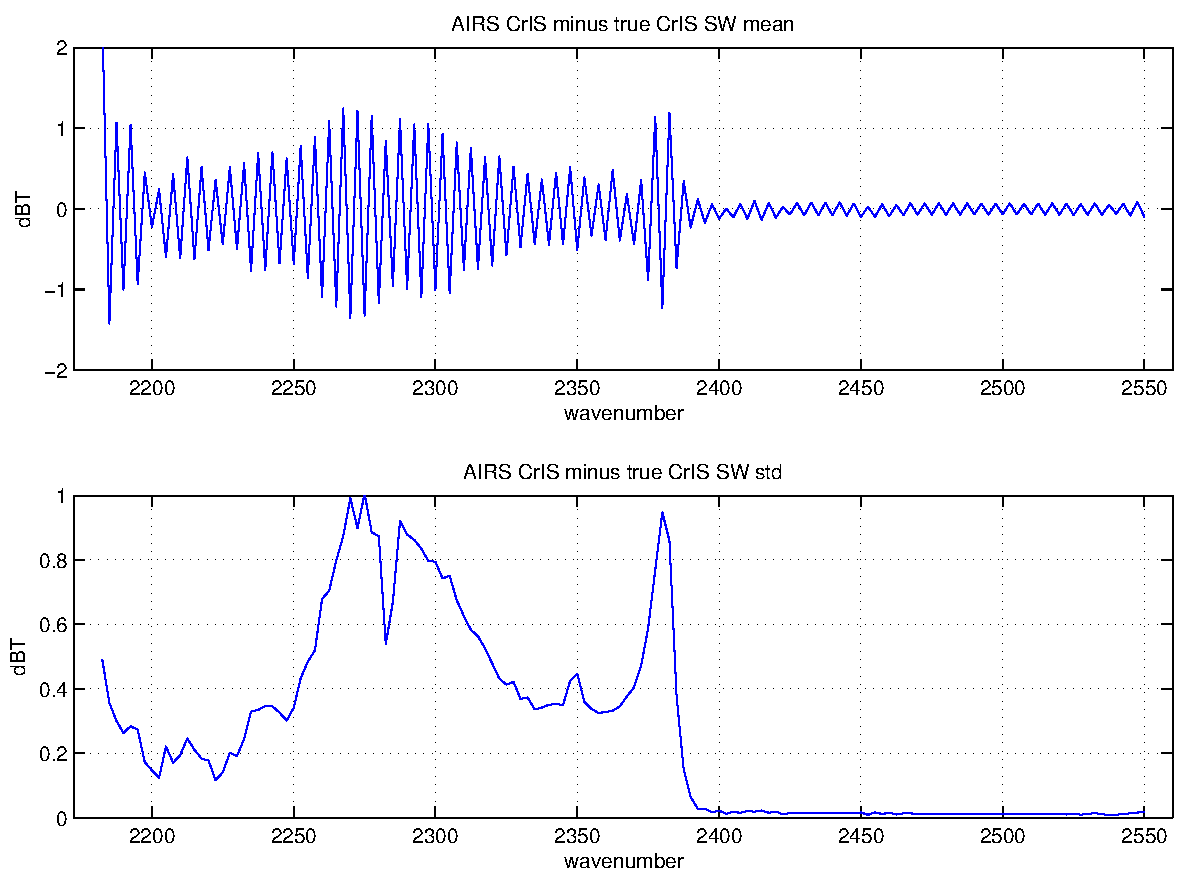
\includegraphics[height=8cm]{figures/airs_cris_diff_SW_noap.pdf}
  \caption{Mean and standard deviation of unapodized {\airs} {\cris}
    minus true {\cris}, for the {\cris} SW band }
  \label{acswd}
\end{figure}

\begin{figure}
  \centering
  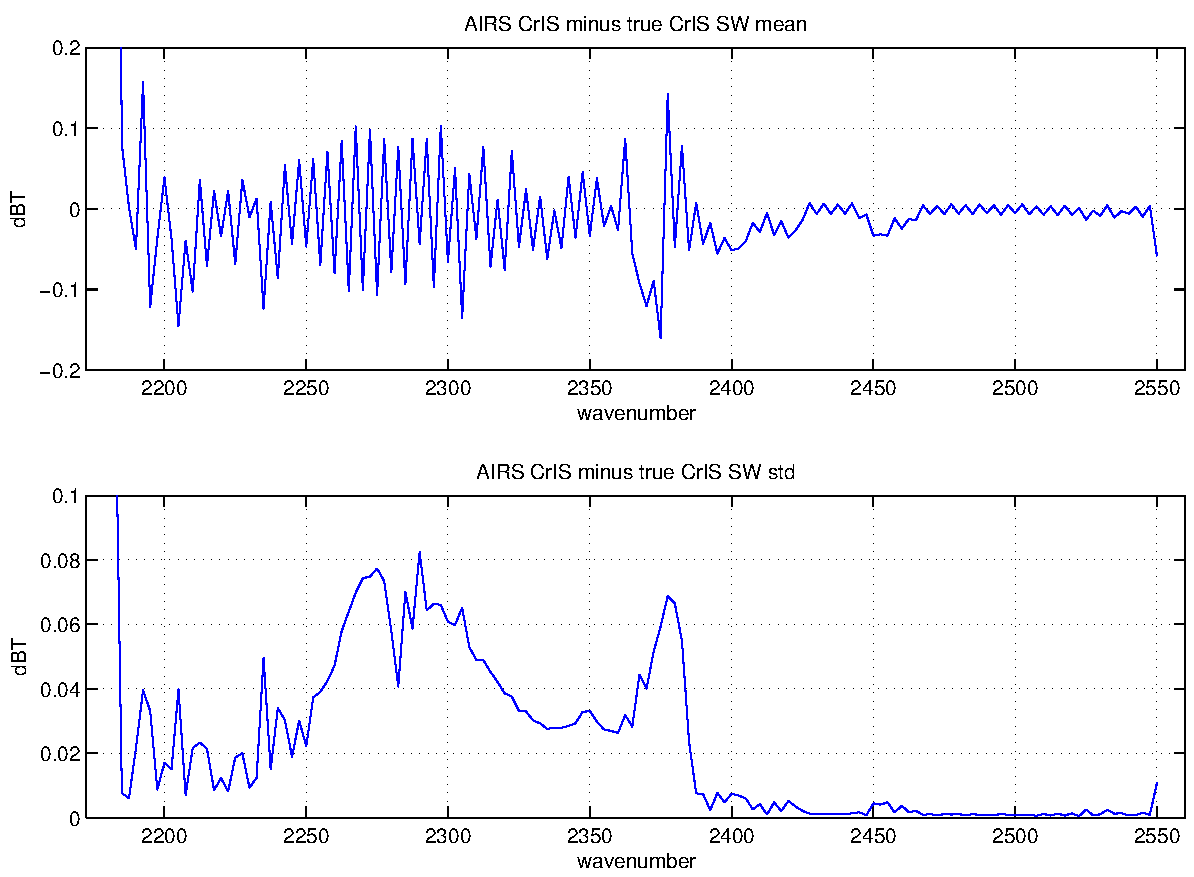
\includegraphics[height=8cm]{figures/airs_cris_diff_SW_hamm.pdf}
  \caption{Mean and standard deviation of Hamming apodized {\airs}
      {\cris} minus true {\cris}, for the {\cris} SW band }
  \label{acswdh}
\end{figure}

\FloatBarrier

\section{High resolution CrIS to AIRS}

The {\cris} to {\airs} translation differs in that we construct the
intermediate representation at the 0.1 {\wn} {\airs} SRF resolution
by double Fourier interpolation, as the {\cris} user grid sinc ILS
does not allow for deconvolution.  For each {\cris} band, the steps
in the translation are as follows,

\begin{itemize}
  \item find the {\airs} and {\cris} band intersection

  \item interpolate the {\cris} channel radiances to the intermediate
    grid 

   \item convolve the 0.1 {\wn} intermediate representation with either
    the {\airs} L1b or L1c SRFs
 
\end{itemize}

Note that there is no bandpass filtering used in this translation.
For example in the LW we simply interpolate the full span of the
{\cris} user grid (plus any guard channels) to the intermediate
representation.  Adding a rolloff inside the user grid would improve
residuals near the band edges but would mean dropping channels from
the translation.

Figure \ref{caspec} shows true {\cris}, true {\airs}, interpolated
{\cris}, and {\cris} {\airs}.  Figure \ref{cazoom} shows details
from 660 to 680 {\wn}.  We do not see the resolution enhancement in
the intermediate representation that we got with the {\iasi} and
{\airs} deconvolutions.  Figure \ref{cadiff} shows {\cris} {\airs}
minus true {\airs}.  The residual is quite large in comparison with
the other translations.

\begin{figure}
  \centering
  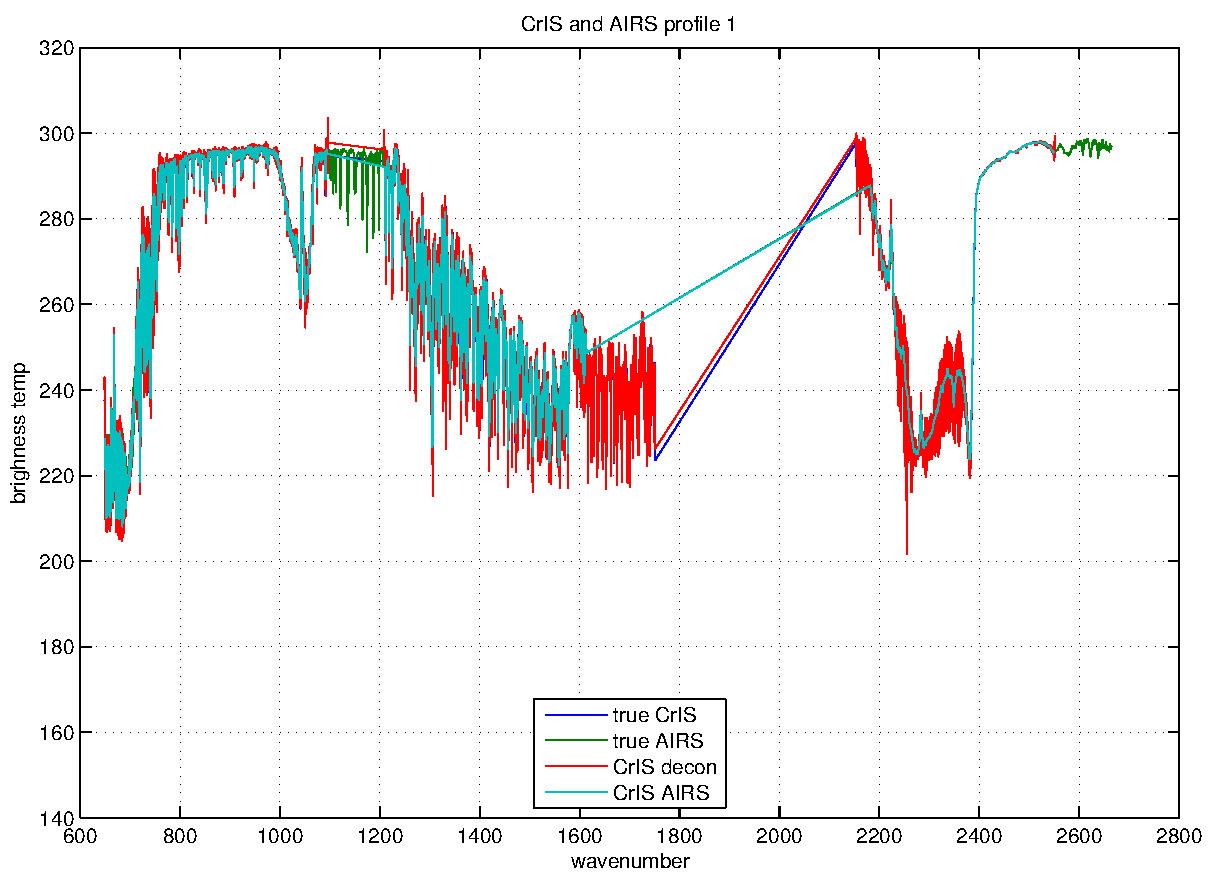
\includegraphics[height=8cm]{figures/cris_airs_spec.pdf}
  \caption{true {\cris}, true {\airs}, interpolated {\cris}, and
    {\cris} {\airs} }
  \label{caspec}
\end{figure}

\begin{figure}
  \centering
  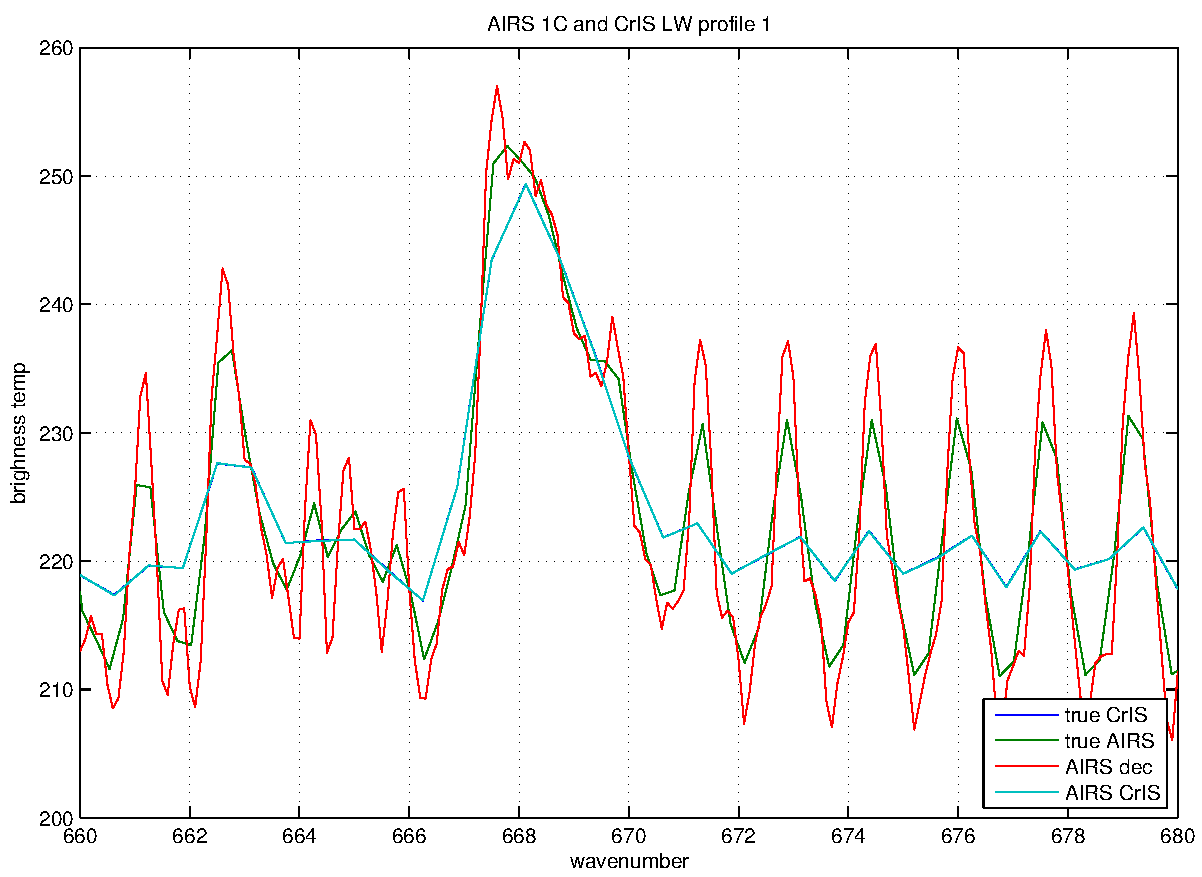
\includegraphics[height=8cm]{figures/cris_airs_zoom.pdf}
  \caption{true {\cris}, true {\airs}, interpolated {\cris}, and
    {\cris} {\airs}, detail}
  \label{cazoom}
\end{figure}

\begin{figure}
  \centering
  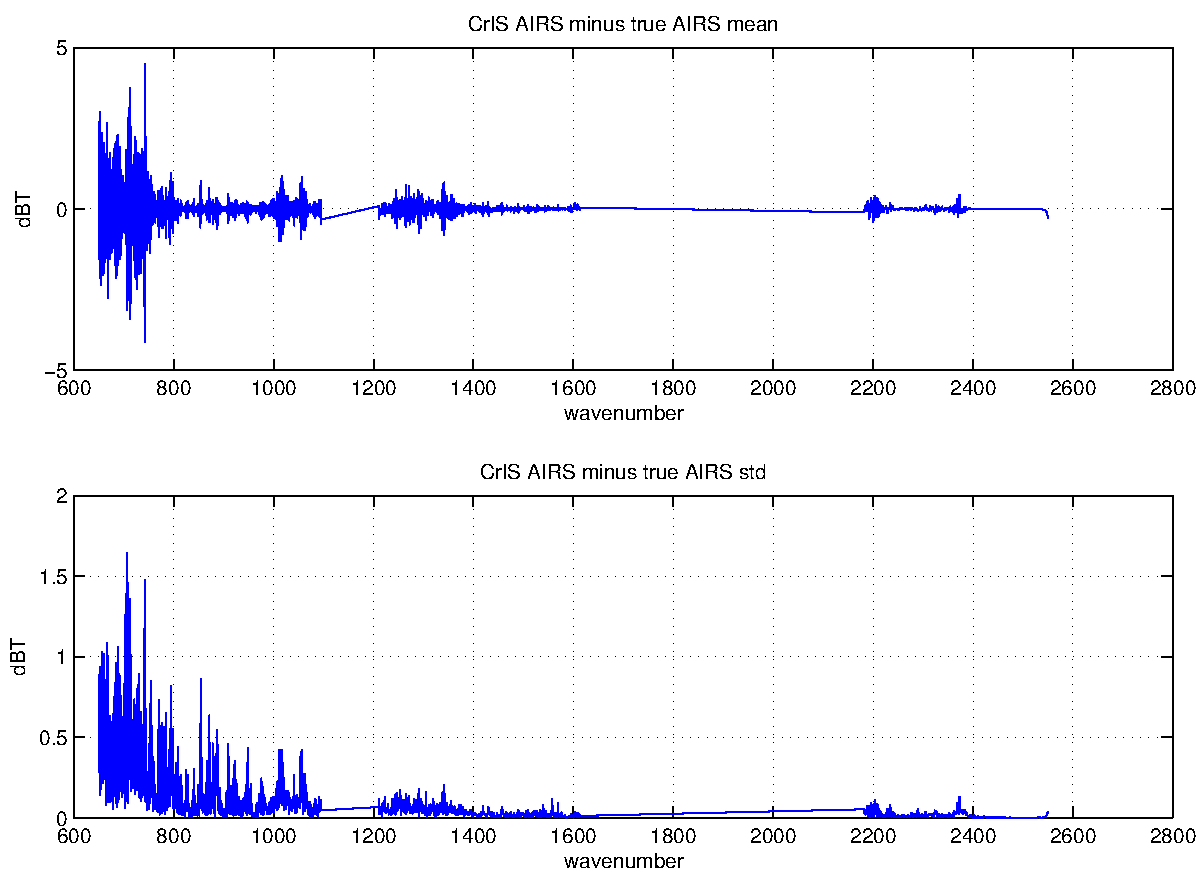
\includegraphics[height=8cm]{figures/cris_airs_diff.pdf}
  \caption{Mean and standard deviation of {\cris} {\airs} minus true
    {\airs}}
  \label{cadiff}
\end{figure}

\FloatBarrier

\section{AIRS Deconvolution}
\label{decon}

\renewcommand{\vec}[1]{\mathbf{#1}}

% \section{AIRS spectral response functions}

The {\airs} spectral response functions model channel response as 
a function of frequency and associate channels with nominal center
frequencies.  Each {\airs} channel $i$ has an associated spectral
response function or {\srf} $\sigma_i(v)$ such that the channel
radiance $c_i = \int \sigma_i(v)r(v)\,dv$, where $r$ is radiance at
frequency $v$.  The center or peak of $\sigma_i$ is the channel
frequency.

Suppose we have $n$ channels and a frequency grid $\vec v$ of $k$
points spanning the domains of the functions $\sigma_i$.  The grid
step size for our applications is often 0.0025 {\wn}, the kcarta
resolution.  Let $S_k$ be an $n\times k$ array such that $s_{i,j} =
\sigma_i(v_j)/w_i$, where $w_i = \sum_j \sigma_i(v_j)$, that is
where row $i$ is $\sigma_i(v)$ tabulated at the grid $\vec v$ and
normalized so the row sum is 1.  If the channel centers are in
increasing order $S_k$ is banded, and if they are not too close the
rows are linearly independent.  $S_k$ is a linear transform whose
domain is radiance at the grid $\vec v$ and whose range is channel
radiances.  If $r$ is radiance at the grid $\vec v$, then $c = S_k r$
gives a good approximation of the channel radiances $c_i = 
\int\sigma_i(v)r(v)\,dv$.

In practice this is how we convolve kcarta or other simulated
radiances to get {\airs} channel radiances.  We construct $S_k$
either explicitly or implicitly from {\airs} {\srf} tabulations.
The matrix $S_k$ in the former case is large but managable with a
banded or sparse representation.

Suppose we have $S_k$ and channel radiances $c$ and want to find
$r$, that is, to deconvolve $c$.  Consider the linear system $S_k x
= c$.  Since $n < k$ for the kcarta grid mentioned above this is
underdetermined, with infinitely many solutions.  We could add
constraints, take a pseudo-inverse, consider a new matrix $S_b$ with
columns tabulated at some coarser grid, or some combination of the
above.  We consider two cases, $S_a$ with SRFs tabulated at the
{\airs} channel grid, and $S_b$ with {\srf}s at an intermediate
grid, typically 0.1 {\wn}, the approximate resolution of the {\srf}
measurements.

\subsection{Deconvolution to the AIRS channel grid}

Let $\vec v_a = v_1,v_2,\ldots,v_n$ be channel center frequencies
associated with a set of {\srf}s.  Similar to $S_k$, let $S_a$ be an
$n\times n$ array where row $i$ is $\sigma_i(v)$ tabulated at the
$v_a$ grid, with rows normalized to 1.  If $r$ is radiance at the
grid $\vec v_a$, then $c = S_a r$ is a rough approximation of
$\int\sigma_i(v)r(v)\,dv$.

Consider the linear system $S_a x = c$, similar to the case 
$S_k x = c$ above, where we are given $S_a$ and channel signals $c$
and want to find radiances $x$.  Since $S_a$ is an $n \times n$
matrix we might hope to solve for $r$.  However in practice there
are problems.  If we take $\vec v_a$ as the standard AIRS L1b
channel set, we find $S_a$ is poorly conditioned, without a usable
inverse.  This is due to the L1b channel spacing, which because of
module overlaps is quite variable, with the closest channels only
0.0036 {\wn} apart.

If we use the the linear function $g(v) = 4\cdot 10^{-4} \cdot v -
0.04$, where $v$ is frequency, as a lower bound on the acceptable
channel spacing, we drop about 64 out of the 2378 L1b channels and
the condition number of $S_a$ is much improved, to around 30.  With
the partly synthetic L1c channel set, $g(v)$ drops only 4 channels
and $\hbox{cond}(S_a)$ is about 250, still low enough to get a
usable inverse.  The higher condition number for the L1c channel set
is not surprising since the extra channels are synthesized from the
L1b set.  

\subsection{Deconvolution to the SRF tabulation grid}

We now consider deconvolution to an intermediate grid, 0.1 {\wn},
the resolution of the tabulated {\airs} {\srf}s.  Let $\vec v_b =
v_1,v_2,\ldots,v_m$ be a 0.1 {\wn} grid spanning the domains of the
functions $\sigma_i$.  Similar to $S_k$, let $S_b$ be an $n\times m$
array where row $i$ is $\sigma_i(v)$ tabulated at the $\vec v_m$
grid, with rows normalized to~1.  If $r$ is radiance at the $\vec
v_b$ grid, then $c = S_b r$ is still a reasonable approximation of
$\int\sigma_i(v)r(v)\,dv$.

Consider the linear system $S_b x = c$, similar to the case 
$S_k x = c$ above, where we are given $S_b$ and channel signals $c$
and want to find radiances $x$.  Since $n < m < k$, as with $S_k$
the system will be underdetermined but more manageable because $m$
is approximately 40 times less than $k$.  After trying several
approaches we settled on a Moore-Penrose pseudoinverse $S_b^{-1}$ of
$S_b$.  Given that, $x = S_b^{-1} c$ gives us deconvolved radiances
at the {\srf} tabulation grid.  This is what we use for the {\airs}
to {\cris} translation in section \ref{airs2cris}.

The {\airs} deconvolution gives a significant resolution enhancement.
Figure \ref{dsinc} shows LW detail of deconvolved {\airs} together
with kcarta radiances convolved directly to a 0.2 {\wn} sinc ILS.
Figure \ref{dbasis} shows a typical basis function for the {\airs}
deconvolution.  This is simply a column of the pseudo-inverse
$S_b^{-1}$.

\begin{figure}
  \centering
  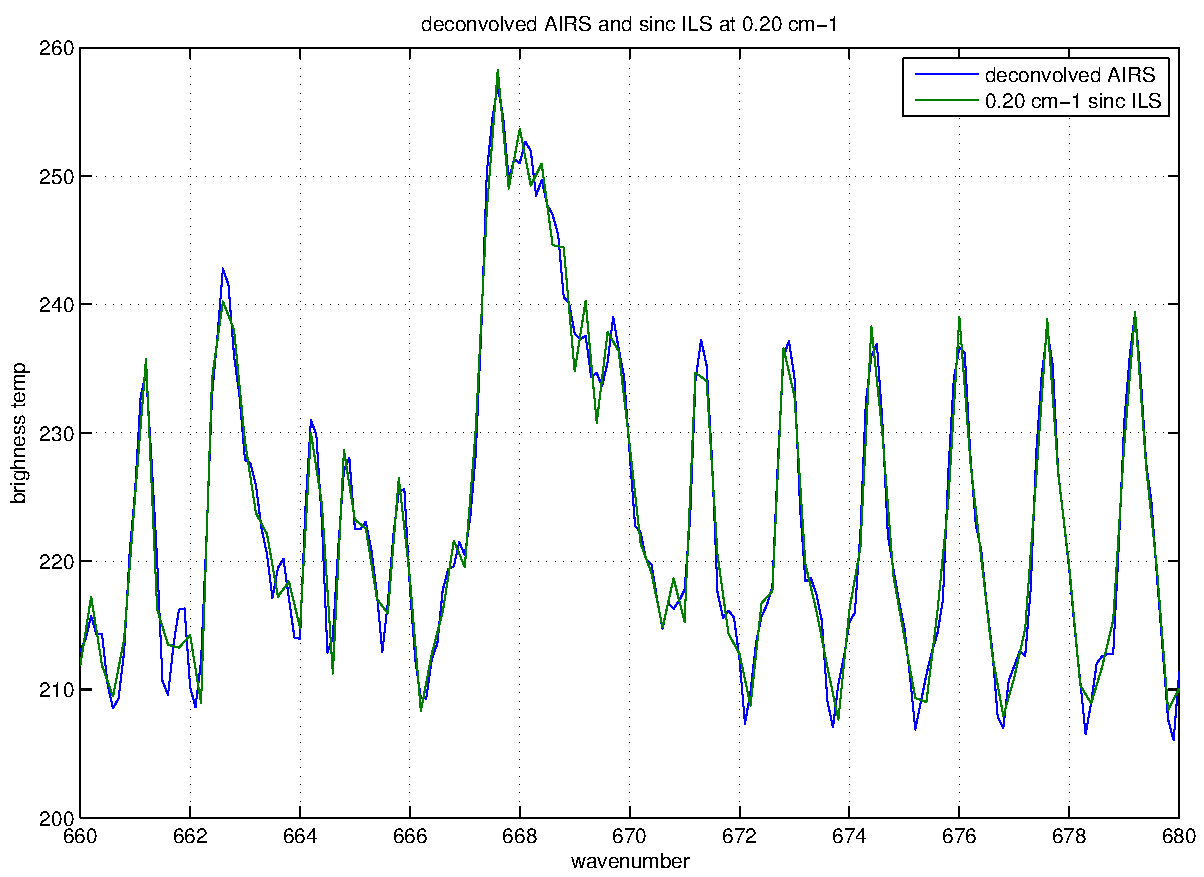
\includegraphics[height=8cm]{figures/airs_decon_res.pdf}
  \caption{deconvolved {\airs} and kcarta radiances convolved to a
    sinc ILS at 0.2 {\wn}}
  \label{dsinc}
\end{figure}

\begin{figure}
  \centering
  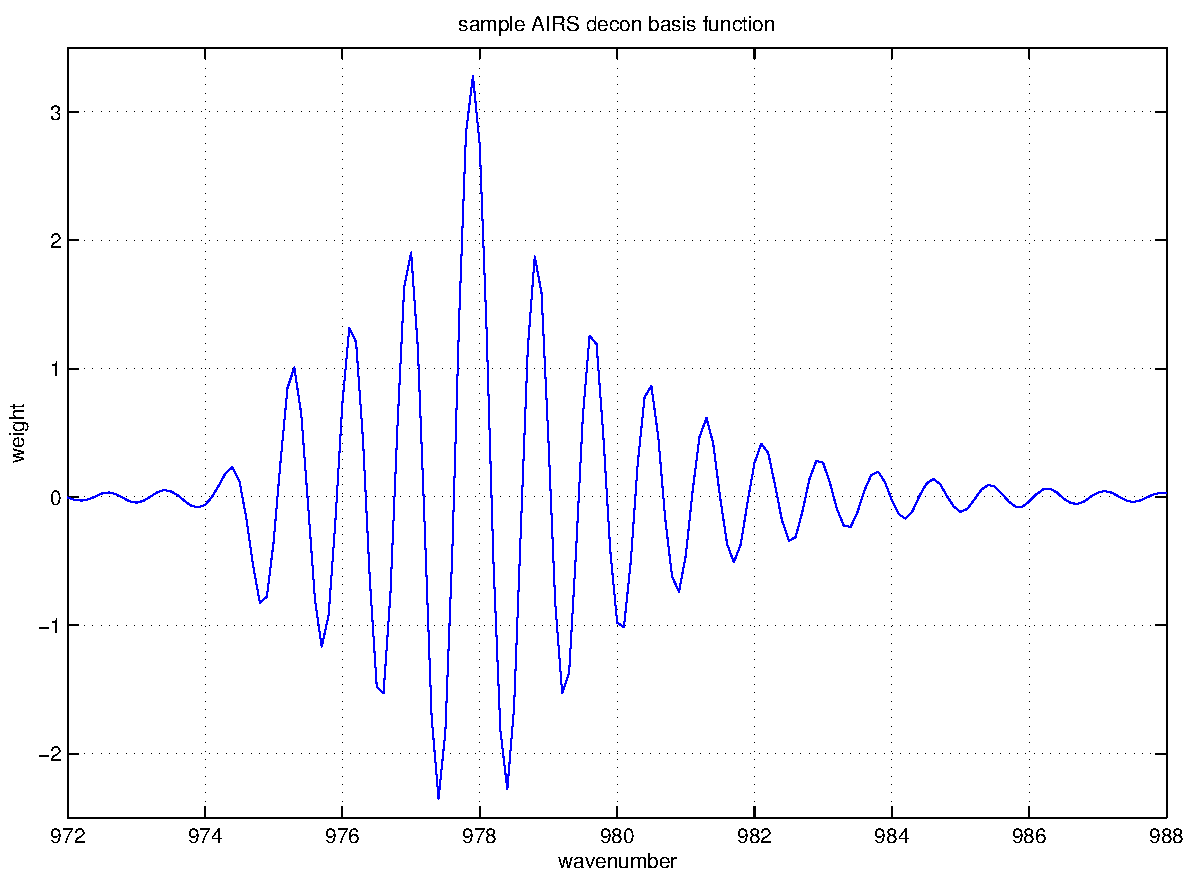
\includegraphics[height=8cm]{figures/airs_decon_basis.pdf}
  \caption{typical basis function for deconvolved {\airs} radiances}
  \label{dbasis}
\end{figure}

\begin{figure}
  \centering
  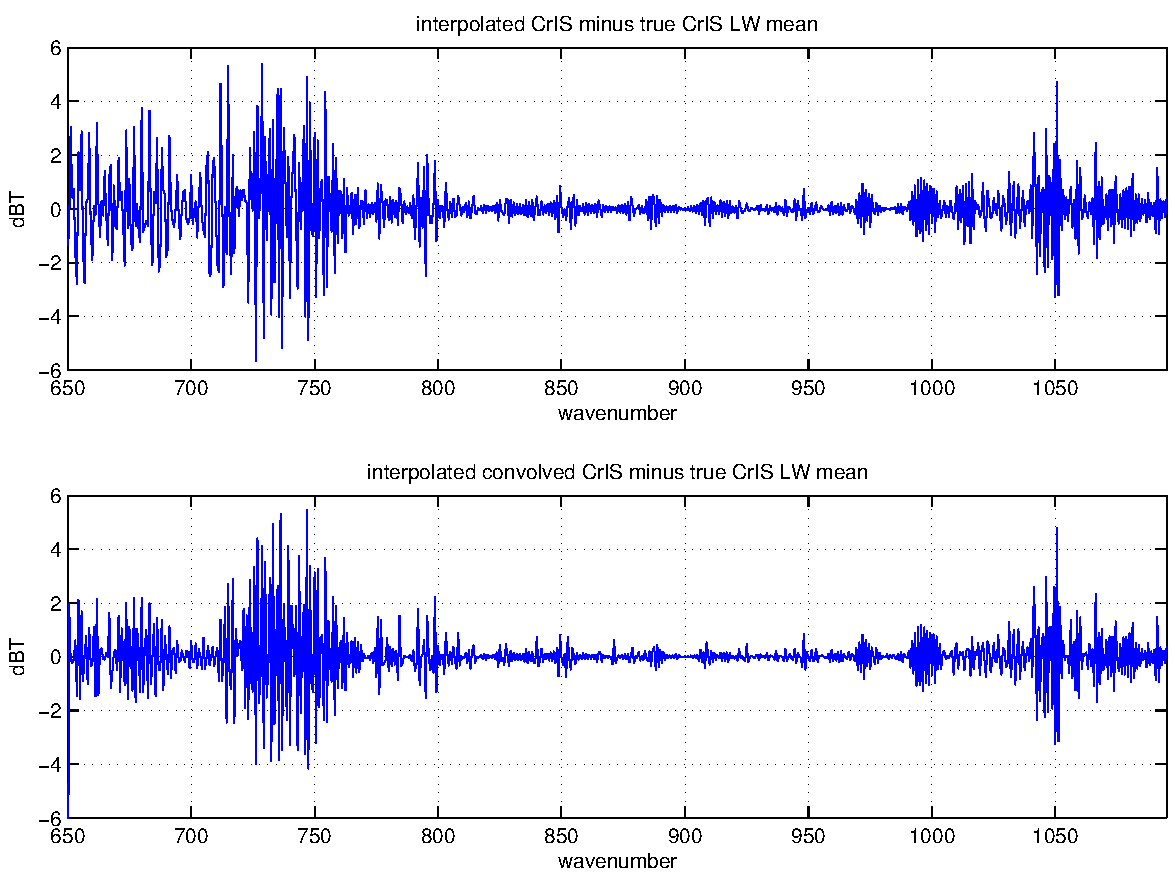
\includegraphics[height=8cm]{figures/airs_cris_intp_LW.pdf}
  \caption{simple interpolation and interpolation with convolution, 
    for the {\cris} LW band}
  \label{intpLW}
\end{figure}

\begin{figure}
  \centering
  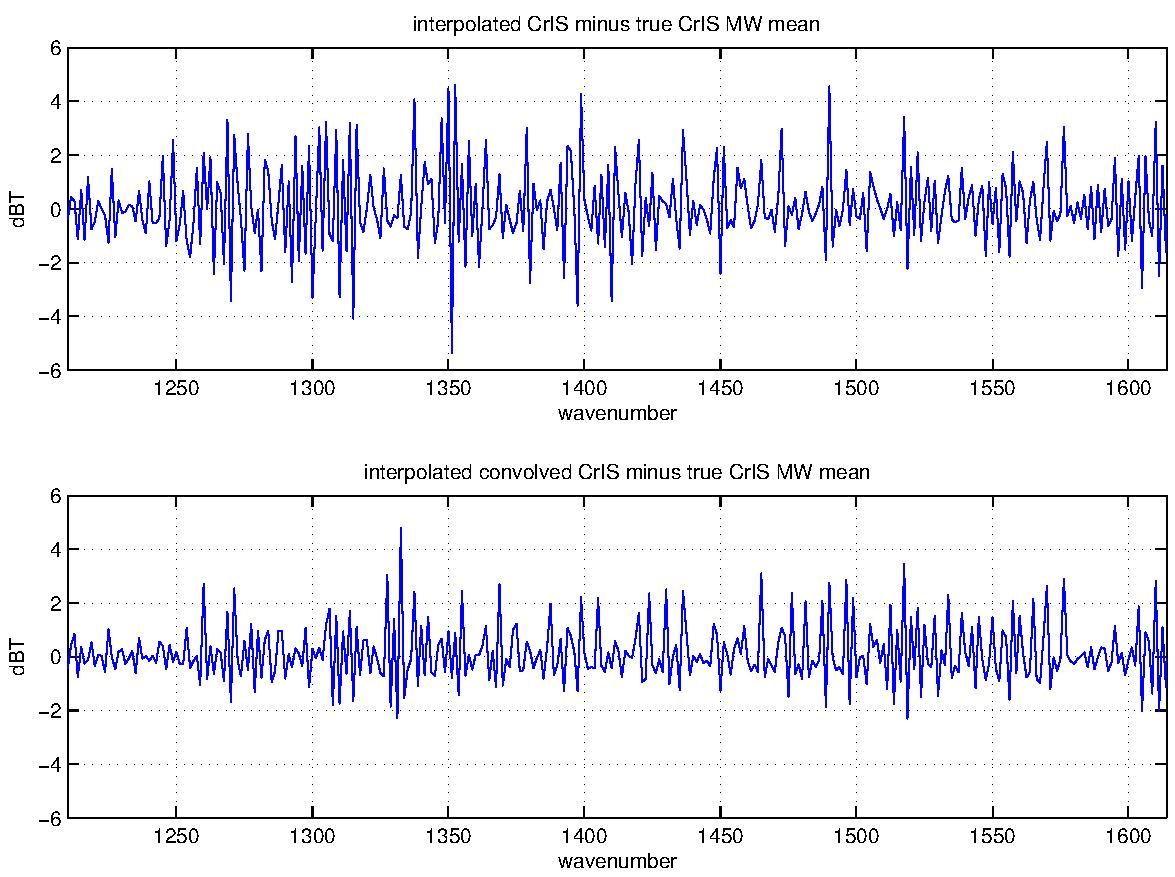
\includegraphics[height=8cm]{figures/airs_cris_intp_MW.pdf}
  \caption{simple interpolation and interpolation with convolution, 
    for the {\cris} MW band}
  \label{intpMW}
\end{figure}

\begin{figure}
  \centering
  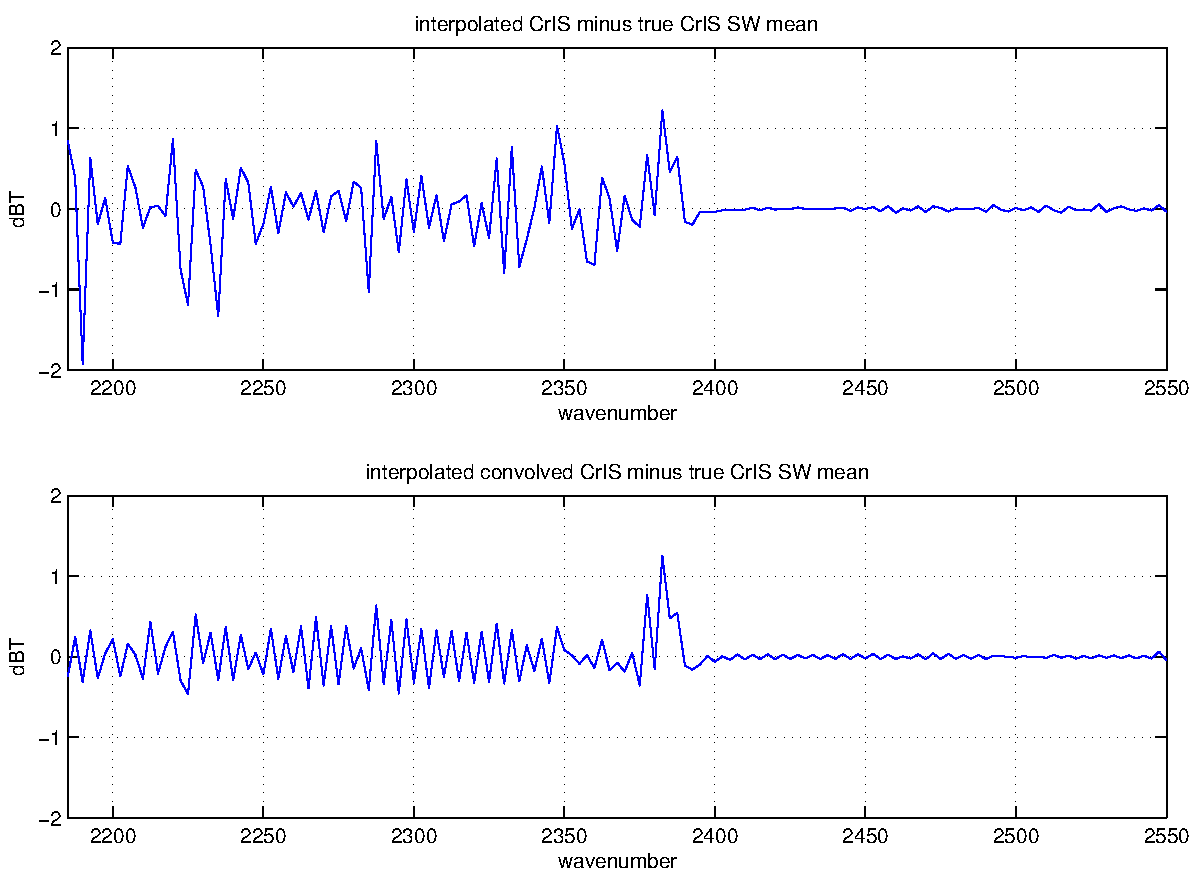
\includegraphics[height=8cm]{figures/airs_cris_intp_SW.pdf}
  \caption{simple interpolation and interpolation with convolution, 
    for the {\cris} SW band}
  \label{intpSW}
\end{figure}

For the {\airs} to {\cris} translation deconvolution works better
than both simple interpolation and interpolation (rather than
deconvolution) to an intermediate grid followed by convolution to
{\cris} radiances.  For the first case we start with true {\airs} and
interpolate radiances directly to the {\cris} user grid with a cubic
spline.  For the second we interpolate true {\airs} to the 0.1 {\wn}
intermediate grid with a cubic spline and then convolve this to the
use {\cris} user grid.

Figure \ref{intpLW} shows interpolated {\cris} minus true {\cris}
for both interpolation tests for the LW band, without any
apodization.  While the two-step interpolation works a little better
than the simple spline, both residuals are significantly larger than
for the translation with deconvolution shown in figure \ref{aclwd}.
Figures \ref{intpMW} and \ref{intpSW} show similar results for the
MW and SW bands.  Deconvolution is significantly better for the MW,
(figure \ref{acmwd}) while the comparison is less clear for the SW
(figure\ref{acswd}).  Comparisons with Hamming apodization show the
residuals with deconvolution are significantly less for all three
bands.

% \FloatBarrier
% 
% \subsection{Notes}
% 
% \begin{itemize}
%   
%   \item Another potential application of the {\airs} deconvolution 
%     is to shift {\airs} SRFs to a more regular reference set, by
%     applying the reference set to the intermediate representation.
% 
%   \item The work evolved as described above, with deconvolution to
%     the AIRS channel grid a key step in getting deconvolution to the
%     SRF tabulation grid to work.  But rather than the AIRS channel
%     grid it might be simpler to deconvolve to $n$ regularly spaced
%     points spanning the SRF domains, and check the condition number
%     and get the channel spacing from that.
% 
%   \item It may be possible to use a sinc basis for the intermediate
%     representation and turn the deconvolution from an under- to an
%     over-determined system that can be solved by regression.  I have
%     notes on this but didn't pursue it because the pseudo-inverse
%     based deconvolution was working fairly well.
% 
% \end{itemize}

\end{document}

